% lecture1.tex -- GENERATED by build_L1.py from L1_numbers.json; do not edit by hand.
\documentclass[10pt,aspectratio=169,t]{beamer}
% =============================================================================
% emqa_preamble.tex -- shared Beamer preamble of Energy Markets Quantitative Analysis (EMQA)
% Used by every lecture: lectures/Lk/lecturek.tex does
%   \documentclass[10pt,aspectratio=169,t]{beamer}
%   % =============================================================================
% emqa_preamble.tex -- shared Beamer preamble of Energy Markets Quantitative Analysis (EMQA)
% Used by every lecture: lectures/Lk/lecturek.tex does
%   \documentclass[10pt,aspectratio=169,t]{beamer}
%   % =============================================================================
% emqa_preamble.tex -- shared Beamer preamble of Energy Markets Quantitative Analysis (EMQA)
% Used by every lecture: lectures/Lk/lecturek.tex does
%   \documentclass[10pt,aspectratio=169,t]{beamer}
%   \input{../common/emqa_preamble}
%   \emqalecture{k}{Lecture title}
% Logos live in lectures/common/logos/, charts in lectures/Lk/charts/.
% Do NOT add \hfuzz / \vfuzz / \hbadness here: overfull boxes must be fixed, not hidden.
% =============================================================================

\usetheme{default}
\setbeamersize{text margin left=7mm, text margin right=7mm}

% ---------------------------------------------------------------- packages
\usepackage[utf8]{inputenc}
\usepackage[T1]{fontenc}
\usepackage{lmodern}
\usepackage{amsmath, amssymb}
\usepackage{mathtools}
\usepackage{bm}
\usepackage{tikz}
\usetikzlibrary{arrows.meta, positioning, calc, shapes.misc}
\usepackage{booktabs}
\usepackage{array}
\usepackage{graphicx}
\usepackage{colortbl}
\usepackage{xcolor}
\usepackage{multicol}
\hypersetup{colorlinks=true, linkcolor=MainBlue, urlcolor=MainBlue, citecolor=MainBlue}
\graphicspath{{../common/logos/}}   % charts are included with their language folder: charts/en/, charts/ro/

% ---------------------------------------------------------------- colours
\definecolor{MainBlue}{RGB}{26, 58, 110}
\definecolor{IDAred}{RGB}{205, 0, 0}
\definecolor{DarkGray}{RGB}{51, 51, 51}
\definecolor{FooterGray}{RGB}{100, 100, 100}
\definecolor{BlockGray}{RGB}{236, 238, 242}
\definecolor{KeynoteGray}{RGB}{218, 218, 218}
\definecolor{Crimson}{RGB}{190, 40, 50}
\definecolor{Forest}{RGB}{30, 110, 50}
\definecolor{Bitter}{RGB}{214, 150, 20}
% chart palette (same hex values as lectures/common/emqa_plot.py)
\definecolor{SerRO}{HTML}{2A78D6}
\definecolor{SerDE}{HTML}{EB6834}
\definecolor{SerHU}{HTML}{1BAF7A}
\definecolor{SerBG}{HTML}{EDA100}

\setbeamertemplate{background}{%
  \begin{tikzpicture}[remember picture, overlay]
    \shade[shading=axis, shading angle=315, top color=white, bottom color=KeynoteGray]
      (current page.south west) rectangle (current page.north east);
  \end{tikzpicture}}
\setbeamercolor{background canvas}{bg=}
\setbeamercolor{structure}{fg=MainBlue}
\setbeamercolor{normal text}{fg=DarkGray}
\setbeamercolor{title}{fg=IDAred}
\setbeamercolor{frametitle}{fg=IDAred, bg=}
\setbeamercolor{block title}{bg=MainBlue, fg=white}
\setbeamercolor{block body}{bg=BlockGray, fg=DarkGray}
\setbeamercolor{block title alerted}{bg=Crimson, fg=white}
\setbeamercolor{block body alerted}{bg=Crimson!7, fg=DarkGray}
\setbeamercolor{block title example}{bg=Forest, fg=white}
\setbeamercolor{block body example}{bg=Forest!7, fg=DarkGray}
\setbeamercolor{item}{fg=MainBlue}
\setbeamerfont{frametitle}{size=\large, series=\bfseries}
\setbeamerfont{block title}{size=\small, series=\bfseries}
\setbeamertemplate{blocks}[rounded][shadow=false]
\setbeamertemplate{itemize item}{\color{MainBlue}$\boxdot$}
\setbeamertemplate{itemize subitem}{\color{MainBlue}\scriptsize$\blacktriangleright$}
% compact two-level lists: level 1 = main point, level 2 = details (no text outside bullets)
\setbeamerfont{itemize/enumerate subbody}{size=\footnotesize}
\setlength{\leftmargini}{1.1em}
\setlength{\leftmarginii}{1.1em}
\setbeamertemplate{itemize/enumerate body begin}{\setlength{\topsep}{0pt}\setlength{\partopsep}{0pt}\setlength{\parskip}{0pt}}
\setbeamertemplate{itemize/enumerate subbody begin}{\setlength{\topsep}{0pt}\setlength{\partopsep}{0pt}\setlength{\itemsep}{0pt}\vspace{-0.4ex}}

\setbeamertemplate{enumerate item}{\color{MainBlue}\insertenumlabel.}
\setlength{\leftmargini}{1.3em}
\setlength{\leftmarginii}{1.2em}
\setbeamertemplate{navigation symbols}{}
\setbeamertemplate{section in toc}{\color{MainBlue}$\blacktriangleright$~\inserttocsection}
\setbeamertemplate{caption}{\raggedright\insertcaption\par}
% frame subtitle = precise citation line under the claim title (Weron style)
\setbeamerfont{framesubtitle}{size=\footnotesize}
\setbeamercolor{framesubtitle}{fg=FooterGray}
% outline that reappears at every section with the current section highlighted
\setbeamertemplate{section in toc shaded}[default][35]
\setbeamertemplate{subsection in toc shaded}[default][35]
\setbeamertemplate{subsection in toc}{\leavevmode\leftskip=2.2em\color{DarkGray}\small\inserttocsubsection\par}
\AtBeginSection[]{{\begin{frame}{\txtoutline}\vspace{2mm}\small
  \tableofcontents[currentsection,hideothersubsections]\end{frame}}}

% ---------------------------------------------------------------- head and foot
\setbeamertemplate{headline}{%
  \vskip10pt%
  \hbox to \paperwidth{\hskip0.5cm%
    {\small\color{FooterGray}\renewcommand{\hyperlink}[2]{##2}\insertsectionhead}%
    \hfill\textcolor{FooterGray}{\small\insertframenumber}\hskip0.5cm}%
  \vskip4pt{\color{FooterGray}\hrule height 0.4pt}}
% footer as in the other courses (MFM, SFM): course name on the left, small sparkline on the right
\setbeamertemplate{footline}{%
  {\color{FooterGray}\hrule height 0.4pt}\vskip4pt%
  \hbox to \paperwidth{\hskip0.5cm%
    \textcolor{FooterGray}{\small\txtcourse}%
    \hfill\raisebox{-0.1em}{\begin{tikzpicture}[x=0.08em, y=0.08em, line width=0.4pt]
      \draw[FooterGray] (0,3) -- (1,4) -- (2,3.5) -- (3,5) -- (4,4) -- (5,6) -- (6,5.5) -- (7,4) -- (8,5) -- (9,7) -- (10,6) -- (11,5) -- (12,6.5) -- (13,8) -- (14,7) -- (15,6) -- (16,7.5) -- (17,9) -- (18,8) -- (19,7) -- (20,8.5) -- (21,10) -- (22,9) -- (23,8) -- (24,9.5);
    \end{tikzpicture}}\hskip0.5cm}%
  \vskip6pt}

% ---------------------------------------------------------------- title page
\defbeamertemplate*{title page}{emqa}[1][]{%
  \vspace{0.15cm}
  \begin{center}
    \href{https://www.ase.ro}{
\includegraphics[height=0.9cm]{ase_logo.png}}\hspace{0.3cm}%
    \href{https://ipe.ro/new}{
\includegraphics[height=0.9cm]{acad_logo.png}}\hspace{0.3cm}%
    \href{https://theida.net}{
\includegraphics[height=0.9cm]{ida_logo.png}}\hspace{0.3cm}%
    \href{https://blockchain-research-center.com}{
\includegraphics[height=0.9cm]{brc_logo.png}}\hspace{0.3cm}%
    \href{https://www.ai4efin.ase.ro}{
\includegraphics[height=0.9cm]{ai4efin_logo.png}}\hspace{0.3cm}%
    \href{https://www.digital-finance-msca.com}{
\includegraphics[height=0.9cm]{msca_logo.png}}%
  \end{center}
  \vspace{0.45cm}
  \begin{center}
    \begin{minipage}{0.1\textwidth}\centering
      \href{https://quantlet.com}{
\includegraphics[height=0.9cm]{ql_logo.png}}\end{minipage}%
    \begin{minipage}{0.78\textwidth}\centering
      {\Large\bfseries\usebeamercolor[fg]{title}\inserttitle}\par\vspace{0.25cm}
      {\large\usebeamercolor[fg]{title}\insertsubtitle}\end{minipage}%
    \begin{minipage}{0.1\textwidth}\centering
      \href{https://quantinar.com}{
\includegraphics[height=0.9cm]{qr_logo.png}}\end{minipage}
  \end{center}
  \vfill
  \hspace{0.4cm}{\bfseries\insertauthor}\par\vspace{0.12cm}
  \hspace{0.4cm}\begin{minipage}[t]{0.92\textwidth}\raggedright\footnotesize\insertinstitute\end{minipage}
  \par\vspace{0.4cm}}

% ---------------------------------------------------------------- lecture metadata
\newcommand{\emqashort}{}
\newcommand{\emqanb}{notebooks}
\newcommand{\emqarepo}{https://github.com/danpele/EMQA/tree/main}
% language-dependent labels (English default; \emqaromanian switches to Romanian, call it before \emqalecture)
\newcommand{\txtcourse}{Energy Markets Quantitative Analysis}
\newcommand{\txtlecture}{Lecture}
\newcommand{\txtoutline}{Outline}
\newcommand{\txtintuition}{In one sentence:}
\newcommand{\txtjob}{In practice:}
\newcommand{\txttry}{Experiment yourself:}
\newcommand{\txtwhere}{where}
\newcommand{\txtsim}{SIMULATED DATA (teaching illustration)}
\newcommand{\txtnbsuffix}{}
\newcommand{\txtinstitute}{Bucharest University of Economic Studies, Department of Statistics and Econometrics\\
    Romanian Academy, Institute for Economic Forecasting\\
    IDA Institute Digital Assets \textbullet\ AI4EFin \textbullet\ MSCA Digital Finance}
\newcommand{\emqaromanian}{%
  \renewcommand{\txtcourse}{Analiza cantitativă a piețelor de energie}%
  \renewcommand{\txtlecture}{Cursul}%
  \renewcommand{\txtoutline}{Cuprins}%
  \renewcommand{\txtintuition}{Pe scurt:}%
  \renewcommand{\txtjob}{În practică:}%
  \renewcommand{\txttry}{Exercițiu practic:}%
  \renewcommand{\txtwhere}{unde}%
  \renewcommand{\txtsim}{DATE SIMULATE (doar pentru ilustrare)}%
  \renewcommand{\txtnbsuffix}{\string_ro}%
  \renewcommand{\txtinstitute}{Academia de Studii Economice din București, Departamentul de Statistică și Econometrie\\
    Academia Română, Institutul de Prognoză Economică\\
    IDA Institute Digital Assets \textbullet\ AI4EFin \textbullet\ MSCA Digital Finance}}
\newcommand{\emqalecture}[2]{%
  \renewcommand{\emqashort}{\txtlecture\ #1}%
  \renewcommand{\emqanb}{notebooks/L#1\string_notebook\txtnbsuffix.ipynb}%
  \title[EMQA]{\txtcourse}%
  \subtitle{\txtlecture\ #1: #2}%
  \author{Prof.\ dr.\ Daniel Traian PELE}%
  \institute{\txtinstitute}%
  \date{}}

% ---------------------------------------------------------------- teaching blocks (MBA clarity rule)
% \intuition{one plain sentence}  ->  formula with every symbol defined  ->  real-data example  ->  \manager{one line}
\newcommand{\intuition}[1]{\begin{itemize}\item {\color{MainBlue}\textbf{\txtintuition}}~#1\end{itemize}\vspace{0.6mm}}
\newcommand{\manager}[1]{\colorbox{Forest!10}{\parbox{\dimexpr\linewidth-2\fboxsep\relax}{\footnotesize
  \begin{itemize}\setlength{\itemsep}{0pt}\item \textbf{\color{Forest}\txtjob}~#1\end{itemize}}}}
% Experiment yourself: pointer to the matching notebook section
\newcommand{\tryit}[1]{{\scriptsize\href{\emqarepo/\emqanb}{%
  \raisebox{-0.15em}{
\includegraphics[height=0.85em]{ql_logo.png}}\,\textbf{\txttry}~\color{MainBlue}#1}}}
% bottom row: manager line (left) + experiment pointer (right), pinned to the bottom of the frame
\newcommand{\bottomrow}[2]{\par\vfill\noindent\begin{minipage}[b]{0.72\linewidth}#1\end{minipage}\hfill
  \begin{minipage}[b]{0.26\linewidth}\raggedleft #2\end{minipage}\par\vspace{0.5mm}}
\newcommand{\where}[1]{{\footnotesize\textbf{\txtwhere}~#1\par}}

% ---------------------------------------------------------------- helpers
% chart source line under a figure: \chartsource{Source ...; period ...}
\newcommand{\chartsource}[1]{\par\vspace{1pt}{\scriptsize\color{FooterGray}#1\par}}
% link to code: \quantlet{label}{path inside the repo}
\newcommand{\quantlet}[2]{\par\vspace{1pt}\hfill\href{\emqarepo/#2}{%
  \raisebox{-0.15em}{
\includegraphics[height=0.75em]{ql_logo.png}}\textcolor{MainBlue}{\scriptsize\ #1}}}
\newcommand{\simlabel}{\colorbox{Crimson!12}{\scriptsize\bfseries\color{Crimson}\txtsim}}
\newcommand{\E}{\mathbb{E}}
\newcommand{\Var}{\operatorname{Var}}
\newcommand{\Cov}{\operatorname{Cov}}
\newcommand{\Corr}{\operatorname{Corr}}
\newcommand{\asinh}{\operatorname{asinh}}
\newcommand{\iid}{\overset{\text{i.i.d.}}{\sim}}
\newcommand{\EUR}{EUR}

%   \emqalecture{k}{Lecture title}
% Logos live in lectures/common/logos/, charts in lectures/Lk/charts/.
% Do NOT add \hfuzz / \vfuzz / \hbadness here: overfull boxes must be fixed, not hidden.
% =============================================================================

\usetheme{default}
\setbeamersize{text margin left=7mm, text margin right=7mm}

% ---------------------------------------------------------------- packages
\usepackage[utf8]{inputenc}
\usepackage[T1]{fontenc}
\usepackage{lmodern}
\usepackage{amsmath, amssymb}
\usepackage{mathtools}
\usepackage{bm}
\usepackage{tikz}
\usetikzlibrary{arrows.meta, positioning, calc, shapes.misc}
\usepackage{booktabs}
\usepackage{array}
\usepackage{graphicx}
\usepackage{colortbl}
\usepackage{xcolor}
\usepackage{multicol}
\hypersetup{colorlinks=true, linkcolor=MainBlue, urlcolor=MainBlue, citecolor=MainBlue}
\graphicspath{{../common/logos/}}   % charts are included with their language folder: charts/en/, charts/ro/

% ---------------------------------------------------------------- colours
\definecolor{MainBlue}{RGB}{26, 58, 110}
\definecolor{IDAred}{RGB}{205, 0, 0}
\definecolor{DarkGray}{RGB}{51, 51, 51}
\definecolor{FooterGray}{RGB}{100, 100, 100}
\definecolor{BlockGray}{RGB}{236, 238, 242}
\definecolor{KeynoteGray}{RGB}{218, 218, 218}
\definecolor{Crimson}{RGB}{190, 40, 50}
\definecolor{Forest}{RGB}{30, 110, 50}
\definecolor{Bitter}{RGB}{214, 150, 20}
% chart palette (same hex values as lectures/common/emqa_plot.py)
\definecolor{SerRO}{HTML}{2A78D6}
\definecolor{SerDE}{HTML}{EB6834}
\definecolor{SerHU}{HTML}{1BAF7A}
\definecolor{SerBG}{HTML}{EDA100}

\setbeamertemplate{background}{%
  \begin{tikzpicture}[remember picture, overlay]
    \shade[shading=axis, shading angle=315, top color=white, bottom color=KeynoteGray]
      (current page.south west) rectangle (current page.north east);
  \end{tikzpicture}}
\setbeamercolor{background canvas}{bg=}
\setbeamercolor{structure}{fg=MainBlue}
\setbeamercolor{normal text}{fg=DarkGray}
\setbeamercolor{title}{fg=IDAred}
\setbeamercolor{frametitle}{fg=IDAred, bg=}
\setbeamercolor{block title}{bg=MainBlue, fg=white}
\setbeamercolor{block body}{bg=BlockGray, fg=DarkGray}
\setbeamercolor{block title alerted}{bg=Crimson, fg=white}
\setbeamercolor{block body alerted}{bg=Crimson!7, fg=DarkGray}
\setbeamercolor{block title example}{bg=Forest, fg=white}
\setbeamercolor{block body example}{bg=Forest!7, fg=DarkGray}
\setbeamercolor{item}{fg=MainBlue}
\setbeamerfont{frametitle}{size=\large, series=\bfseries}
\setbeamerfont{block title}{size=\small, series=\bfseries}
\setbeamertemplate{blocks}[rounded][shadow=false]
\setbeamertemplate{itemize item}{\color{MainBlue}$\boxdot$}
\setbeamertemplate{itemize subitem}{\color{MainBlue}\scriptsize$\blacktriangleright$}
% compact two-level lists: level 1 = main point, level 2 = details (no text outside bullets)
\setbeamerfont{itemize/enumerate subbody}{size=\footnotesize}
\setlength{\leftmargini}{1.1em}
\setlength{\leftmarginii}{1.1em}
\setbeamertemplate{itemize/enumerate body begin}{\setlength{\topsep}{0pt}\setlength{\partopsep}{0pt}\setlength{\parskip}{0pt}}
\setbeamertemplate{itemize/enumerate subbody begin}{\setlength{\topsep}{0pt}\setlength{\partopsep}{0pt}\setlength{\itemsep}{0pt}\vspace{-0.4ex}}

\setbeamertemplate{enumerate item}{\color{MainBlue}\insertenumlabel.}
\setlength{\leftmargini}{1.3em}
\setlength{\leftmarginii}{1.2em}
\setbeamertemplate{navigation symbols}{}
\setbeamertemplate{section in toc}{\color{MainBlue}$\blacktriangleright$~\inserttocsection}
\setbeamertemplate{caption}{\raggedright\insertcaption\par}
% frame subtitle = precise citation line under the claim title (Weron style)
\setbeamerfont{framesubtitle}{size=\footnotesize}
\setbeamercolor{framesubtitle}{fg=FooterGray}
% outline that reappears at every section with the current section highlighted
\setbeamertemplate{section in toc shaded}[default][35]
\setbeamertemplate{subsection in toc shaded}[default][35]
\setbeamertemplate{subsection in toc}{\leavevmode\leftskip=2.2em\color{DarkGray}\small\inserttocsubsection\par}
\AtBeginSection[]{{\begin{frame}{\txtoutline}\vspace{2mm}\small
  \tableofcontents[currentsection,hideothersubsections]\end{frame}}}

% ---------------------------------------------------------------- head and foot
\setbeamertemplate{headline}{%
  \vskip10pt%
  \hbox to \paperwidth{\hskip0.5cm%
    {\small\color{FooterGray}\renewcommand{\hyperlink}[2]{##2}\insertsectionhead}%
    \hfill\textcolor{FooterGray}{\small\insertframenumber}\hskip0.5cm}%
  \vskip4pt{\color{FooterGray}\hrule height 0.4pt}}
% footer as in the other courses (MFM, SFM): course name on the left, small sparkline on the right
\setbeamertemplate{footline}{%
  {\color{FooterGray}\hrule height 0.4pt}\vskip4pt%
  \hbox to \paperwidth{\hskip0.5cm%
    \textcolor{FooterGray}{\small\txtcourse}%
    \hfill\raisebox{-0.1em}{\begin{tikzpicture}[x=0.08em, y=0.08em, line width=0.4pt]
      \draw[FooterGray] (0,3) -- (1,4) -- (2,3.5) -- (3,5) -- (4,4) -- (5,6) -- (6,5.5) -- (7,4) -- (8,5) -- (9,7) -- (10,6) -- (11,5) -- (12,6.5) -- (13,8) -- (14,7) -- (15,6) -- (16,7.5) -- (17,9) -- (18,8) -- (19,7) -- (20,8.5) -- (21,10) -- (22,9) -- (23,8) -- (24,9.5);
    \end{tikzpicture}}\hskip0.5cm}%
  \vskip6pt}

% ---------------------------------------------------------------- title page
\defbeamertemplate*{title page}{emqa}[1][]{%
  \vspace{0.15cm}
  \begin{center}
    \href{https://www.ase.ro}{
\includegraphics[height=0.9cm]{ase_logo.png}}\hspace{0.3cm}%
    \href{https://ipe.ro/new}{
\includegraphics[height=0.9cm]{acad_logo.png}}\hspace{0.3cm}%
    \href{https://theida.net}{
\includegraphics[height=0.9cm]{ida_logo.png}}\hspace{0.3cm}%
    \href{https://blockchain-research-center.com}{
\includegraphics[height=0.9cm]{brc_logo.png}}\hspace{0.3cm}%
    \href{https://www.ai4efin.ase.ro}{
\includegraphics[height=0.9cm]{ai4efin_logo.png}}\hspace{0.3cm}%
    \href{https://www.digital-finance-msca.com}{
\includegraphics[height=0.9cm]{msca_logo.png}}%
  \end{center}
  \vspace{0.45cm}
  \begin{center}
    \begin{minipage}{0.1\textwidth}\centering
      \href{https://quantlet.com}{
\includegraphics[height=0.9cm]{ql_logo.png}}\end{minipage}%
    \begin{minipage}{0.78\textwidth}\centering
      {\Large\bfseries\usebeamercolor[fg]{title}\inserttitle}\par\vspace{0.25cm}
      {\large\usebeamercolor[fg]{title}\insertsubtitle}\end{minipage}%
    \begin{minipage}{0.1\textwidth}\centering
      \href{https://quantinar.com}{
\includegraphics[height=0.9cm]{qr_logo.png}}\end{minipage}
  \end{center}
  \vfill
  \hspace{0.4cm}{\bfseries\insertauthor}\par\vspace{0.12cm}
  \hspace{0.4cm}\begin{minipage}[t]{0.92\textwidth}\raggedright\footnotesize\insertinstitute\end{minipage}
  \par\vspace{0.4cm}}

% ---------------------------------------------------------------- lecture metadata
\newcommand{\emqashort}{}
\newcommand{\emqanb}{notebooks}
\newcommand{\emqarepo}{https://github.com/danpele/EMQA/tree/main}
% language-dependent labels (English default; \emqaromanian switches to Romanian, call it before \emqalecture)
\newcommand{\txtcourse}{Energy Markets Quantitative Analysis}
\newcommand{\txtlecture}{Lecture}
\newcommand{\txtoutline}{Outline}
\newcommand{\txtintuition}{In one sentence:}
\newcommand{\txtjob}{In practice:}
\newcommand{\txttry}{Experiment yourself:}
\newcommand{\txtwhere}{where}
\newcommand{\txtsim}{SIMULATED DATA (teaching illustration)}
\newcommand{\txtnbsuffix}{}
\newcommand{\txtinstitute}{Bucharest University of Economic Studies, Department of Statistics and Econometrics\\
    Romanian Academy, Institute for Economic Forecasting\\
    IDA Institute Digital Assets \textbullet\ AI4EFin \textbullet\ MSCA Digital Finance}
\newcommand{\emqaromanian}{%
  \renewcommand{\txtcourse}{Analiza cantitativă a piețelor de energie}%
  \renewcommand{\txtlecture}{Cursul}%
  \renewcommand{\txtoutline}{Cuprins}%
  \renewcommand{\txtintuition}{Pe scurt:}%
  \renewcommand{\txtjob}{În practică:}%
  \renewcommand{\txttry}{Exercițiu practic:}%
  \renewcommand{\txtwhere}{unde}%
  \renewcommand{\txtsim}{DATE SIMULATE (doar pentru ilustrare)}%
  \renewcommand{\txtnbsuffix}{\string_ro}%
  \renewcommand{\txtinstitute}{Academia de Studii Economice din București, Departamentul de Statistică și Econometrie\\
    Academia Română, Institutul de Prognoză Economică\\
    IDA Institute Digital Assets \textbullet\ AI4EFin \textbullet\ MSCA Digital Finance}}
\newcommand{\emqalecture}[2]{%
  \renewcommand{\emqashort}{\txtlecture\ #1}%
  \renewcommand{\emqanb}{notebooks/L#1\string_notebook\txtnbsuffix.ipynb}%
  \title[EMQA]{\txtcourse}%
  \subtitle{\txtlecture\ #1: #2}%
  \author{Prof.\ dr.\ Daniel Traian PELE}%
  \institute{\txtinstitute}%
  \date{}}

% ---------------------------------------------------------------- teaching blocks (MBA clarity rule)
% \intuition{one plain sentence}  ->  formula with every symbol defined  ->  real-data example  ->  \manager{one line}
\newcommand{\intuition}[1]{\begin{itemize}\item {\color{MainBlue}\textbf{\txtintuition}}~#1\end{itemize}\vspace{0.6mm}}
\newcommand{\manager}[1]{\colorbox{Forest!10}{\parbox{\dimexpr\linewidth-2\fboxsep\relax}{\footnotesize
  \begin{itemize}\setlength{\itemsep}{0pt}\item \textbf{\color{Forest}\txtjob}~#1\end{itemize}}}}
% Experiment yourself: pointer to the matching notebook section
\newcommand{\tryit}[1]{{\scriptsize\href{\emqarepo/\emqanb}{%
  \raisebox{-0.15em}{
\includegraphics[height=0.85em]{ql_logo.png}}\,\textbf{\txttry}~\color{MainBlue}#1}}}
% bottom row: manager line (left) + experiment pointer (right), pinned to the bottom of the frame
\newcommand{\bottomrow}[2]{\par\vfill\noindent\begin{minipage}[b]{0.72\linewidth}#1\end{minipage}\hfill
  \begin{minipage}[b]{0.26\linewidth}\raggedleft #2\end{minipage}\par\vspace{0.5mm}}
\newcommand{\where}[1]{{\footnotesize\textbf{\txtwhere}~#1\par}}

% ---------------------------------------------------------------- helpers
% chart source line under a figure: \chartsource{Source ...; period ...}
\newcommand{\chartsource}[1]{\par\vspace{1pt}{\scriptsize\color{FooterGray}#1\par}}
% link to code: \quantlet{label}{path inside the repo}
\newcommand{\quantlet}[2]{\par\vspace{1pt}\hfill\href{\emqarepo/#2}{%
  \raisebox{-0.15em}{
\includegraphics[height=0.75em]{ql_logo.png}}\textcolor{MainBlue}{\scriptsize\ #1}}}
\newcommand{\simlabel}{\colorbox{Crimson!12}{\scriptsize\bfseries\color{Crimson}\txtsim}}
\newcommand{\E}{\mathbb{E}}
\newcommand{\Var}{\operatorname{Var}}
\newcommand{\Cov}{\operatorname{Cov}}
\newcommand{\Corr}{\operatorname{Corr}}
\newcommand{\asinh}{\operatorname{asinh}}
\newcommand{\iid}{\overset{\text{i.i.d.}}{\sim}}
\newcommand{\EUR}{EUR}

%   \emqalecture{k}{Lecture title}
% Logos live in lectures/common/logos/, charts in lectures/Lk/charts/.
% Do NOT add \hfuzz / \vfuzz / \hbadness here: overfull boxes must be fixed, not hidden.
% =============================================================================

\usetheme{default}
\setbeamersize{text margin left=7mm, text margin right=7mm}

% ---------------------------------------------------------------- packages
\usepackage[utf8]{inputenc}
\usepackage[T1]{fontenc}
\usepackage{lmodern}
\usepackage{amsmath, amssymb}
\usepackage{mathtools}
\usepackage{bm}
\usepackage{tikz}
\usetikzlibrary{arrows.meta, positioning, calc, shapes.misc}
\usepackage{booktabs}
\usepackage{array}
\usepackage{graphicx}
\usepackage{colortbl}
\usepackage{xcolor}
\usepackage{multicol}
\hypersetup{colorlinks=true, linkcolor=MainBlue, urlcolor=MainBlue, citecolor=MainBlue}
\graphicspath{{../common/logos/}}   % charts are included with their language folder: charts/en/, charts/ro/

% ---------------------------------------------------------------- colours
\definecolor{MainBlue}{RGB}{26, 58, 110}
\definecolor{IDAred}{RGB}{205, 0, 0}
\definecolor{DarkGray}{RGB}{51, 51, 51}
\definecolor{FooterGray}{RGB}{100, 100, 100}
\definecolor{BlockGray}{RGB}{236, 238, 242}
\definecolor{KeynoteGray}{RGB}{218, 218, 218}
\definecolor{Crimson}{RGB}{190, 40, 50}
\definecolor{Forest}{RGB}{30, 110, 50}
\definecolor{Bitter}{RGB}{214, 150, 20}
% chart palette (same hex values as lectures/common/emqa_plot.py)
\definecolor{SerRO}{HTML}{2A78D6}
\definecolor{SerDE}{HTML}{EB6834}
\definecolor{SerHU}{HTML}{1BAF7A}
\definecolor{SerBG}{HTML}{EDA100}

\setbeamertemplate{background}{%
  \begin{tikzpicture}[remember picture, overlay]
    \shade[shading=axis, shading angle=315, top color=white, bottom color=KeynoteGray]
      (current page.south west) rectangle (current page.north east);
  \end{tikzpicture}}
\setbeamercolor{background canvas}{bg=}
\setbeamercolor{structure}{fg=MainBlue}
\setbeamercolor{normal text}{fg=DarkGray}
\setbeamercolor{title}{fg=IDAred}
\setbeamercolor{frametitle}{fg=IDAred, bg=}
\setbeamercolor{block title}{bg=MainBlue, fg=white}
\setbeamercolor{block body}{bg=BlockGray, fg=DarkGray}
\setbeamercolor{block title alerted}{bg=Crimson, fg=white}
\setbeamercolor{block body alerted}{bg=Crimson!7, fg=DarkGray}
\setbeamercolor{block title example}{bg=Forest, fg=white}
\setbeamercolor{block body example}{bg=Forest!7, fg=DarkGray}
\setbeamercolor{item}{fg=MainBlue}
\setbeamerfont{frametitle}{size=\large, series=\bfseries}
\setbeamerfont{block title}{size=\small, series=\bfseries}
\setbeamertemplate{blocks}[rounded][shadow=false]
\setbeamertemplate{itemize item}{\color{MainBlue}$\boxdot$}
\setbeamertemplate{itemize subitem}{\color{MainBlue}\scriptsize$\blacktriangleright$}
% compact two-level lists: level 1 = main point, level 2 = details (no text outside bullets)
\setbeamerfont{itemize/enumerate subbody}{size=\footnotesize}
\setlength{\leftmargini}{1.1em}
\setlength{\leftmarginii}{1.1em}
\setbeamertemplate{itemize/enumerate body begin}{\setlength{\topsep}{0pt}\setlength{\partopsep}{0pt}\setlength{\parskip}{0pt}}
\setbeamertemplate{itemize/enumerate subbody begin}{\setlength{\topsep}{0pt}\setlength{\partopsep}{0pt}\setlength{\itemsep}{0pt}\vspace{-0.4ex}}

\setbeamertemplate{enumerate item}{\color{MainBlue}\insertenumlabel.}
\setlength{\leftmargini}{1.3em}
\setlength{\leftmarginii}{1.2em}
\setbeamertemplate{navigation symbols}{}
\setbeamertemplate{section in toc}{\color{MainBlue}$\blacktriangleright$~\inserttocsection}
\setbeamertemplate{caption}{\raggedright\insertcaption\par}
% frame subtitle = precise citation line under the claim title (Weron style)
\setbeamerfont{framesubtitle}{size=\footnotesize}
\setbeamercolor{framesubtitle}{fg=FooterGray}
% outline that reappears at every section with the current section highlighted
\setbeamertemplate{section in toc shaded}[default][35]
\setbeamertemplate{subsection in toc shaded}[default][35]
\setbeamertemplate{subsection in toc}{\leavevmode\leftskip=2.2em\color{DarkGray}\small\inserttocsubsection\par}
\AtBeginSection[]{{\begin{frame}{\txtoutline}\vspace{2mm}\small
  \tableofcontents[currentsection,hideothersubsections]\end{frame}}}

% ---------------------------------------------------------------- head and foot
\setbeamertemplate{headline}{%
  \vskip10pt%
  \hbox to \paperwidth{\hskip0.5cm%
    {\small\color{FooterGray}\renewcommand{\hyperlink}[2]{##2}\insertsectionhead}%
    \hfill\textcolor{FooterGray}{\small\insertframenumber}\hskip0.5cm}%
  \vskip4pt{\color{FooterGray}\hrule height 0.4pt}}
% footer as in the other courses (MFM, SFM): course name on the left, small sparkline on the right
\setbeamertemplate{footline}{%
  {\color{FooterGray}\hrule height 0.4pt}\vskip4pt%
  \hbox to \paperwidth{\hskip0.5cm%
    \textcolor{FooterGray}{\small\txtcourse}%
    \hfill\raisebox{-0.1em}{\begin{tikzpicture}[x=0.08em, y=0.08em, line width=0.4pt]
      \draw[FooterGray] (0,3) -- (1,4) -- (2,3.5) -- (3,5) -- (4,4) -- (5,6) -- (6,5.5) -- (7,4) -- (8,5) -- (9,7) -- (10,6) -- (11,5) -- (12,6.5) -- (13,8) -- (14,7) -- (15,6) -- (16,7.5) -- (17,9) -- (18,8) -- (19,7) -- (20,8.5) -- (21,10) -- (22,9) -- (23,8) -- (24,9.5);
    \end{tikzpicture}}\hskip0.5cm}%
  \vskip6pt}

% ---------------------------------------------------------------- title page
\defbeamertemplate*{title page}{emqa}[1][]{%
  \vspace{0.15cm}
  \begin{center}
    \href{https://www.ase.ro}{
\includegraphics[height=0.9cm]{ase_logo.png}}\hspace{0.3cm}%
    \href{https://ipe.ro/new}{
\includegraphics[height=0.9cm]{acad_logo.png}}\hspace{0.3cm}%
    \href{https://theida.net}{
\includegraphics[height=0.9cm]{ida_logo.png}}\hspace{0.3cm}%
    \href{https://blockchain-research-center.com}{
\includegraphics[height=0.9cm]{brc_logo.png}}\hspace{0.3cm}%
    \href{https://www.ai4efin.ase.ro}{
\includegraphics[height=0.9cm]{ai4efin_logo.png}}\hspace{0.3cm}%
    \href{https://www.digital-finance-msca.com}{
\includegraphics[height=0.9cm]{msca_logo.png}}%
  \end{center}
  \vspace{0.45cm}
  \begin{center}
    \begin{minipage}{0.1\textwidth}\centering
      \href{https://quantlet.com}{
\includegraphics[height=0.9cm]{ql_logo.png}}\end{minipage}%
    \begin{minipage}{0.78\textwidth}\centering
      {\Large\bfseries\usebeamercolor[fg]{title}\inserttitle}\par\vspace{0.25cm}
      {\large\usebeamercolor[fg]{title}\insertsubtitle}\end{minipage}%
    \begin{minipage}{0.1\textwidth}\centering
      \href{https://quantinar.com}{
\includegraphics[height=0.9cm]{qr_logo.png}}\end{minipage}
  \end{center}
  \vfill
  \hspace{0.4cm}{\bfseries\insertauthor}\par\vspace{0.12cm}
  \hspace{0.4cm}\begin{minipage}[t]{0.92\textwidth}\raggedright\footnotesize\insertinstitute\end{minipage}
  \par\vspace{0.4cm}}

% ---------------------------------------------------------------- lecture metadata
\newcommand{\emqashort}{}
\newcommand{\emqanb}{notebooks}
\newcommand{\emqarepo}{https://github.com/danpele/EMQA/tree/main}
% language-dependent labels (English default; \emqaromanian switches to Romanian, call it before \emqalecture)
\newcommand{\txtcourse}{Energy Markets Quantitative Analysis}
\newcommand{\txtlecture}{Lecture}
\newcommand{\txtoutline}{Outline}
\newcommand{\txtintuition}{In one sentence:}
\newcommand{\txtjob}{In practice:}
\newcommand{\txttry}{Experiment yourself:}
\newcommand{\txtwhere}{where}
\newcommand{\txtsim}{SIMULATED DATA (teaching illustration)}
\newcommand{\txtnbsuffix}{}
\newcommand{\txtinstitute}{Bucharest University of Economic Studies, Department of Statistics and Econometrics\\
    Romanian Academy, Institute for Economic Forecasting\\
    IDA Institute Digital Assets \textbullet\ AI4EFin \textbullet\ MSCA Digital Finance}
\newcommand{\emqaromanian}{%
  \renewcommand{\txtcourse}{Analiza cantitativă a piețelor de energie}%
  \renewcommand{\txtlecture}{Cursul}%
  \renewcommand{\txtoutline}{Cuprins}%
  \renewcommand{\txtintuition}{Pe scurt:}%
  \renewcommand{\txtjob}{În practică:}%
  \renewcommand{\txttry}{Exercițiu practic:}%
  \renewcommand{\txtwhere}{unde}%
  \renewcommand{\txtsim}{DATE SIMULATE (doar pentru ilustrare)}%
  \renewcommand{\txtnbsuffix}{\string_ro}%
  \renewcommand{\txtinstitute}{Academia de Studii Economice din București, Departamentul de Statistică și Econometrie\\
    Academia Română, Institutul de Prognoză Economică\\
    IDA Institute Digital Assets \textbullet\ AI4EFin \textbullet\ MSCA Digital Finance}}
\newcommand{\emqalecture}[2]{%
  \renewcommand{\emqashort}{\txtlecture\ #1}%
  \renewcommand{\emqanb}{notebooks/L#1\string_notebook\txtnbsuffix.ipynb}%
  \title[EMQA]{\txtcourse}%
  \subtitle{\txtlecture\ #1: #2}%
  \author{Prof.\ dr.\ Daniel Traian PELE}%
  \institute{\txtinstitute}%
  \date{}}

% ---------------------------------------------------------------- teaching blocks (MBA clarity rule)
% \intuition{one plain sentence}  ->  formula with every symbol defined  ->  real-data example  ->  \manager{one line}
\newcommand{\intuition}[1]{\begin{itemize}\item {\color{MainBlue}\textbf{\txtintuition}}~#1\end{itemize}\vspace{0.6mm}}
\newcommand{\manager}[1]{\colorbox{Forest!10}{\parbox{\dimexpr\linewidth-2\fboxsep\relax}{\footnotesize
  \begin{itemize}\setlength{\itemsep}{0pt}\item \textbf{\color{Forest}\txtjob}~#1\end{itemize}}}}
% Experiment yourself: pointer to the matching notebook section
\newcommand{\tryit}[1]{{\scriptsize\href{\emqarepo/\emqanb}{%
  \raisebox{-0.15em}{
\includegraphics[height=0.85em]{ql_logo.png}}\,\textbf{\txttry}~\color{MainBlue}#1}}}
% bottom row: manager line (left) + experiment pointer (right), pinned to the bottom of the frame
\newcommand{\bottomrow}[2]{\par\vfill\noindent\begin{minipage}[b]{0.72\linewidth}#1\end{minipage}\hfill
  \begin{minipage}[b]{0.26\linewidth}\raggedleft #2\end{minipage}\par\vspace{0.5mm}}
\newcommand{\where}[1]{{\footnotesize\textbf{\txtwhere}~#1\par}}

% ---------------------------------------------------------------- helpers
% chart source line under a figure: \chartsource{Source ...; period ...}
\newcommand{\chartsource}[1]{\par\vspace{1pt}{\scriptsize\color{FooterGray}#1\par}}
% link to code: \quantlet{label}{path inside the repo}
\newcommand{\quantlet}[2]{\par\vspace{1pt}\hfill\href{\emqarepo/#2}{%
  \raisebox{-0.15em}{
\includegraphics[height=0.75em]{ql_logo.png}}\textcolor{MainBlue}{\scriptsize\ #1}}}
\newcommand{\simlabel}{\colorbox{Crimson!12}{\scriptsize\bfseries\color{Crimson}\txtsim}}
\newcommand{\E}{\mathbb{E}}
\newcommand{\Var}{\operatorname{Var}}
\newcommand{\Cov}{\operatorname{Cov}}
\newcommand{\Corr}{\operatorname{Corr}}
\newcommand{\asinh}{\operatorname{asinh}}
\newcommand{\iid}{\overset{\text{i.i.d.}}{\sim}}
\newcommand{\EUR}{EUR}

\emqalecture{1}{Energy Markets and Their Data}
\begin{document}
{\setbeamertemplate{headline}{}\setbeamertemplate{footline}{}
\begin{frame}\titlepage\end{frame}}
% END-FRONT-MATTER

\begin{frame}{Learning objectives}
\small
\begin{itemize}\setlength{\itemsep}{1pt}
  \item Explain how one day-ahead auction sets a price for every hour (now every quarter-hour) and how European market coupling links Romania with its neighbours.
  \item Compute and read the Romanian generation mix from metered data, with its coverage.
  \item Recognise the stylized facts of power prices on real data and choose a transformation that works when prices are zero or negative.
  \item Use the core time-series toolkit and the naive benchmark that every forecast must beat.
  \item Read six current episodes quantitatively, from the dry year 2025 to Bulgaria's new batteries in 2026.
\end{itemize}
\end{frame}

% BEGIN-ABBR

\begin{frame}{Abbreviations (1/2)}
\small
\vspace{-1mm}\begin{columns}[T,onlytextwidth]
\begin{column}{0.49\textwidth}{\scriptsize\renewcommand{\arraystretch}{0.96}\begin{tabular}{@{}>{\bfseries}l@{\ \ }p{0.76\linewidth}@{}}ACER & EU Agency for the Cooperation of Energy Regulators\\
ACF & autocorrelation function\\
ADF & augmented Dickey--Fuller test\\
AIC & Akaike information criterion\\
ANRE & Romanian Energy Regulatory Authority\\
AR & autoregressive model\\
ARX & autoregressive model with exogenous variables\\
bbl & barrel (159 litres)\\
BG & Bulgaria (bidding zone)\\
CEST & Central European Summer Time\\
CET & Central European Time\\
CNCAN & National Commission for Nuclear Activities Control (Romania)\\
DE-LU & Germany--Luxembourg bidding zone\\
DST & daylight saving time\\
ECB & European Central Bank\\
EET & Eastern European Time (Romania)\\\end{tabular}}\end{column}
\begin{column}{0.49\textwidth}{\scriptsize\renewcommand{\arraystretch}{0.96}\begin{tabular}{@{}>{\bfseries}l@{\ \ }p{0.76\linewidth}@{}}ENTSO-E & European Network of Transmission System Operators for Electricity\\
EPEX & EPEX SPOT power exchange\\
EU & European Union\\
EUPHEMIA & Pan-European Hybrid Electricity Market Integration Algorithm\\
EUR & euro\\
EWMA & exponentially weighted moving average\\
GW & gigawatt\\
HAC & heteroskedasticity- and autocorrelation-consistent\\
HU & Hungary (bidding zone)\\
HUPX & Hungarian Power Exchange\\
IBEX & Independent Bulgarian Energy Exchange\\
IDA & intraday auction\\
IQR & interquartile range\\
ISE & Fraunhofer Institute for Solar Energy Systems\\
JAO & Joint Allocation Office\\\end{tabular}}\end{column}
\end{columns}
\end{frame}

\begin{frame}{Abbreviations (2/2)}
\small
\vspace{-1mm}\begin{columns}[T,onlytextwidth]
\begin{column}{0.49\textwidth}{\scriptsize\renewcommand{\arraystretch}{0.96}\begin{tabular}{@{}>{\bfseries}l@{\ \ }p{0.76\linewidth}@{}}JB & Jarque--Bera test\\
KPSS & Kwiatkowski--Phillips--Schmidt--Shin test\\
MA & moving average\\
MAD & median absolute deviation\\
MAE & mean absolute error\\
MMBtu & million British thermal units\\
MTU & market time unit\\
MW & megawatt\\
MWh & megawatt-hour\\
NEMO & Nominated Electricity Market Operator\\
OLS & ordinary least squares\\
OPCOM & Romanian electricity and gas market operator\\
OTC & over the counter (bilateral)\\
PACF & partial autocorrelation function\\
PPA & power purchase agreement\\
PZU & Piața pentru Ziua Următoare (day-ahead market)\\\end{tabular}}\end{column}
\begin{column}{0.49\textwidth}{\scriptsize\renewcommand{\arraystretch}{0.96}\begin{tabular}{@{}>{\bfseries}l@{\ \ }p{0.76\linewidth}@{}}REMIT & EU Regulation 1227/2011 on wholesale energy market integrity and transparency\\
RO & Romania (bidding zone)\\
RON & Romanian leu\\
RoR & run-of-river hydro\\
SDAC & Single Day-Ahead Coupling\\
SES & simple exponential smoothing\\
SIDC & Single Intraday Coupling\\
SMA & simple moving average\\
STL & Seasonal--Trend decomposition using Loess\\
TSO & transmission system operator\\
TTF & Title Transfer Facility (Dutch gas hub)\\
TWh & terawatt-hour\\
USD & US dollar\\
UTC & Coordinated Universal Time\\
YTD & year to date\\\end{tabular}}\end{column}
\end{columns}
\end{frame}

% END-ABBR

\begin{frame}{Real data only: what we use and where it ends}
\framesubtitle{\hfill\tryit{notebook \S1}}
\small

\par\vspace{0.5mm}{\scriptsize \begin{itemize}\setlength{\itemsep}{0pt}
  \item Exchanges: Romanian electricity and gas market operator (OPCOM), Independent Bulgarian Energy Exchange (IBEX), Hungarian Power Exchange (HUPX), European Power Exchange (EPEX SPOT); European Network of Transmission System Operators for Electricity (ENTSO-E).
\end{itemize}}\vspace{-1mm}
{\scriptsize\renewcommand{\arraystretch}{1.0}\setlength{\tabcolsep}{4pt}
\begin{tabular}{@{}p{0.31\textwidth}p{0.11\textwidth}p{0.36\textwidth}p{0.13\textwidth}@{}}\toprule
Series & Frequency & Source & From \\ \midrule
Day-ahead prices: Romania (RO), Bulgaria (BG), Hungary (HU), Germany--Luxembourg (DE-LU) & 15/60 min & energy-charts.info (Fraunhofer ISE); prices of the exchanges above & 2015-01-01 \\
Generation by source and consumption, Romania and Bulgaria & hourly & energy-charts.info, ENTSO-E actual generation & 2015-01 \\
Romanian cross-border physical flows & hourly & energy-charts.info, ENTSO-E & 2015-01-01 \\
Brent crude oil, front-month futures & daily & Yahoo Finance (BZ=F) & 2015-01-02 \\
Title Transfer Facility (TTF) gas, monthly & monthly & World Bank; European Central Bank (ECB) exchange rates & 2015-01 \\
\bottomrule\end{tabular}}
\vspace{0.5mm}
\begin{itemize}\setlength{\itemsep}{1pt}
  \item \textbf{Cut-off: 31 Oct 2026} (last complete month), downloaded 4 Nov 2026
    \begin{itemize}\setlength{\itemsep}{0pt}
      \item ``2026 year to date (YTD)'' always means Jan--Oct 2026.
    \end{itemize}
  \item Missing values stay missing: never interpolated, never counted as zero, and coverage is always reported.
\end{itemize}
\end{frame}


\section{Power markets in Romania and Europe}

\subsection{How the day-ahead auction works}

\begin{frame}{One auction, one price per quarter-hour: where supply meets demand}
\framesubtitle{(Weron, 2014, IJF; Maciejowska, Uniejewski \& Weron, 2023, Oxford Res.\ Enc.)}
\footnotesize
\intuition{Sellers and buyers send price--quantity bids; the exchange finds the price at which energy offered equals energy demanded, and every accepted trade is paid that single price.}
\begin{columns}[T,onlytextwidth]
\begin{column}{0.45\textwidth}
\[ p_t^{*}=\min\big\{p:\ \underbrace{S_t(p)}_{\text{supply curve}}\ \ge\ \underbrace{D_t(p)}_{\text{demand curve}}\big\} \]{\footnotesize\begin{itemize}\setlength{\itemsep}{0pt}
  \item \textbf{\txtwhere}
    \begin{itemize}\setlength{\itemsep}{0pt}
      \item $t$ = delivery quarter-hour (hour before Oct 2025)
      \item $S_t(p)$ = energy offered at prices $\le p$, plants sorted by cost (the \emph{merit order}: renewables and nuclear at the bottom, gas near the top)
      \item $D_t(p)$ = energy bought at prices $\ge p$
      \item $p_t^{*}$ = clearing price, in euro per megawatt-hour (EUR/MWh).
    \end{itemize}
\end{itemize}\par}
\end{column}
\begin{column}{0.52\textwidth}
\begin{itemize}\setlength{\itemsep}{1pt}
  \item \textbf{On our data}: Romania's day-ahead market, Piața pentru Ziua Următoare (PZU), run by the Romanian market operator (OPCOM), cleared on average at 137.45 EUR/MWh in Jan--Oct 2026.
  \item Reservoir hydro bids its ``water value'' (opportunity cost) and often sets the Romanian price.
  \item \textbf{Two extremes}
    \begin{itemize}\setlength{\itemsep}{0pt}
      \item Demand on the steep part: \textbf{spikes}
      \item Inflexible output and sun above demand: \textbf{negative prices}
    \end{itemize}
\end{itemize}
\end{column}
\end{columns}
\par\vfill\manager{on PZU a supplier pays the price of the most expensive plant needed, not the average cost.}\par\vspace{0.5mm}
\end{frame}

\begin{frame}{The merit order: how the price is formed}
\framesubtitle{(Weron, 2014, IJF; Maciejowska, Uniejewski \& Weron, 2023, Oxford Res.\ Enc.)}
\footnotesize
\begin{itemize}\setlength{\itemsep}{1pt}
  \item \textbf{Supply}: sell offers sorted from cheapest to dearest
    \begin{itemize}\setlength{\itemsep}{0pt}
      \item Each producer offers near its marginal cost, the cost of one more MWh
      \item Usual order: wind, solar and nuclear (marginal cost near zero), run-of-river hydro, lignite, gas
      \item Reservoir hydro offers at its water value, the price it expects to get later for the same water
    \end{itemize}
  \item \textbf{Demand}: buy bids sorted from highest to lowest price
    \begin{itemize}\setlength{\itemsep}{0pt}
      \item Most consumption is bought at any price, so the demand curve is almost vertical
    \end{itemize}
  \item \textbf{Price}: set by the last accepted offer, the marginal one
    \begin{itemize}\setlength{\itemsep}{0pt}
      \item Every accepted seller receives it, also those with lower costs
      \item Their difference between price and cost pays for capacity (inframarginal rent)
    \end{itemize}
  \item \textbf{Why prices move}
    \begin{itemize}\setlength{\itemsep}{0pt}
      \item Sun and wind shift the supply to the right: lower price
      \item Evening demand or a missing reactor moves the crossing to the steep, gas-fired part: higher price
    \end{itemize}
\end{itemize}
\par\vfill\manager{the price of a quarter-hour is the cost of its most expensive accepted offer, not the average cost of the system.}\par\vspace{0.5mm}
\end{frame}

\begin{frame}{The merit order on real OPCOM curves, 21 Oct 2026}
\framesubtitle{(OPCOM, PZU aggregated curves)\hfill\tryit{notebook \S1}}
\small
\begin{center}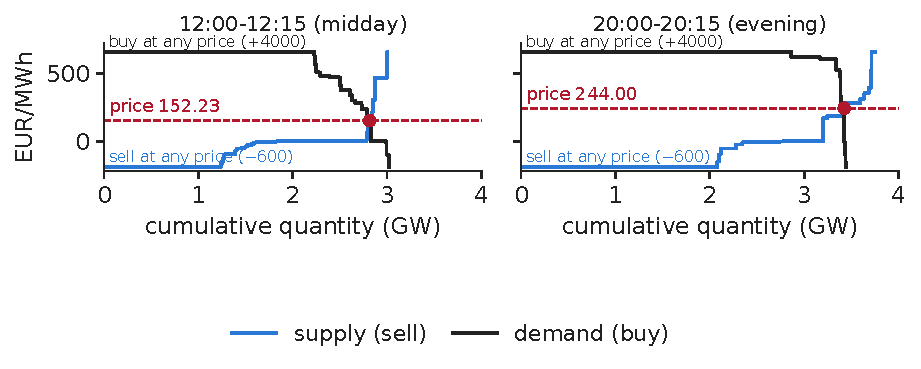
\includegraphics[width=\textwidth,height=0.481\textheight,keepaspectratio]{charts/en/merit_opcom.pdf}\end{center}\vspace{-3mm}
\chartsource{Source: OPCOM, PZU aggregated curves. Data: 2026-10-21, Romanian time; quantities include blocks, hourly orders and net flows.}
\vspace{0.5mm}
\begin{itemize}\setlength{\itemsep}{0pt}
  \item Midday: 2\,333 MW offered at zero or negative prices
    \begin{itemize}\setlength{\itemsep}{0pt}
      \item Price 152.23 EUR/MWh.
    \end{itemize}
  \item Evening: no sun, 1\,054 MW of net imports in the supply
    \begin{itemize}\setlength{\itemsep}{0pt}
      \item Price 244.00 EUR/MWh.
    \end{itemize}
\end{itemize}
\par\vfill\manager{a buyer who can shift consumption from evening to midday pays the lower clearing price.}\par\vspace{0.5mm}
\end{frame}

\begin{frame}{One delivery day, step by step}
\framesubtitle{(Maciejowska, Uniejewski \& Weron, 2023, Oxford Res.\ Enc.; OPCOM; Transelectrica)}
\footnotesize

\begin{center}
\begin{tikzpicture}[x=1cm,y=1cm,
  box/.style={draw=MainBlue,fill=BlockGray,rounded corners=2pt,align=center,text width=3.05cm,minimum height=1.3cm,font=\scriptsize}]
\draw[-{Latex},thick,MainBlue] (0,0) -- (14.5,0);
\node[box] at (1.7,1.05) {\textbf{1. Forward contracts}\\ OPCOM centralised markets, over-the-counter (OTC) deals; weeks to years ahead};
\node[box] at (5.3,1.05) {\textbf{2. PZU bid}\\ gate closure 12:00 Central European Time (CET) on $d-1$ = 13:00 in Bucharest; results published early afternoon};
\node[box] at (8.9,1.05) {\textbf{3. Intraday correction}\\ intraday auctions (IDA) and continuous trading until shortly before delivery};
\node[box] at (12.5,1.05) {\textbf{4. Imbalance}\\ Transelectrica, the transmission system operator (TSO), balances the grid; deviations settled per 15 min};
\foreach \x/\l in {1.7/{weeks--years}, 5.3/{day $d-1$}, 8.9/{$d-1$ and $d$}, 12.5/{day $d$, real time}}
  \node[font=\scriptsize,below] at (\x,-0.05) {\l};
\end{tikzpicture}
\end{center}
\vspace{1mm}
\begin{itemize}\setlength{\itemsep}{1pt}
  \item \textbf{Clocks and money}: Romania runs on Eastern European Time (EET), one hour ahead of CET
    \begin{itemize}\setlength{\itemsep}{0pt}
      \item The Single Day-Ahead Coupling (SDAC) clears in EUR, and OPCOM also publishes prices in Romanian lei (RON).
    \end{itemize}
  \item \textbf{Why the order matters}: each step corrects the previous one
    \begin{itemize}\setlength{\itemsep}{0pt}
      \item What is not covered forward is bought on PZU, and what is still wrong after intraday trading is settled as imbalance.
    \end{itemize}
\end{itemize}
\par\vfill\manager{a trader hedges forward, bids on PZU before 13:00 Bucharest time, fixes forecast errors intraday and pays what is left as imbalance.}\par\vspace{0.5mm}
\end{frame}

\begin{frame}{Who sets the rules: operators, regulators, price limits, disclosure}
\framesubtitle{(OPCOM; ANRE; ACER; Regulation (EU) 1227/2011)}
\footnotesize
\begin{itemize}\setlength{\itemsep}{1pt}
  \item \textbf{Who is who}
    \begin{itemize}\setlength{\itemsep}{0pt}
      \item OPCOM: the Nominated Electricity Market Operator (NEMO); it runs PZU and the intraday market
      \item Transelectrica (TSO): runs the grid in real time and settles imbalances
      \item The Romanian Energy Regulatory Authority (ANRE): sets the national rules and licenses market participants
    \end{itemize}
  \item \textbf{Disclosure}
    \begin{itemize}\setlength{\itemsep}{0pt}
      \item The European Union (EU) Regulation on wholesale energy market integrity and transparency (REMIT): inside information must be published promptly
      \item For example, unplanned outages of large plants; such messages move PZU prices
      \item The EU Agency for the Cooperation of Energy Regulators (ACER) monitors the market for abuse
    \end{itemize}
  \item \textbf{Price limits}
    \begin{itemize}\setlength{\itemsep}{0pt}
      \item SDAC harmonised minimum: $-500$ EUR/MWh; $-600$ for delivery from 29 May 2026 (OPCOM)
      \item A series that touches the floor is censored there: the true willingness to pay was even lower
    \end{itemize}
\end{itemize}
\par\vfill\manager{read REMIT messages before bidding
    \begin{itemize}\setlength{\itemsep}{0pt}
      \item An unplanned outage announced in time changes the PZU price.
    \end{itemize}}\par\vspace{0.5mm}
\end{frame}

\subsection{Market coupling and the 15-minute market time unit}

\begin{frame}{Coupling lets power flow to the higher price until the network limit binds}
\framesubtitle{(Weron, 2014, IJF; JAO; Core flow-based market coupling)}
\footnotesize
\intuition{Europe runs one joint day-ahead auction; cheap zones export to expensive ones until a network limit binds, and only then do prices differ.}
\begin{columns}[T,onlytextwidth]
\begin{column}{0.45\textwidth}
\[ \max\sum_{z}\Big[\underbrace{\textstyle\int_0^{d_z}\!D_z^{-1}}_{\text{buyers' value}}-\underbrace{\textstyle\int_0^{s_z}\!S_z^{-1}}_{\text{sellers' cost}}\Big]\ \text{s.t. }\underbrace{\mathbf{flows}\in\mathcal F}_{\text{network limits}} \]{\footnotesize\begin{itemize}\setlength{\itemsep}{0pt}
  \item \textbf{\txtwhere}
    \begin{itemize}\setlength{\itemsep}{0pt}
      \item $z$ = bidding zone
      \item $d_z, s_z$ = energy bought and sold in $z$
      \item $\mathcal F$ = feasible exchanges
      \item If no limit binds, $p_z=p_{z'}$, otherwise prices separate.
    \end{itemize}
\end{itemize}\par}
\end{column}
\begin{column}{0.52\textwidth}
\begin{itemize}\setlength{\itemsep}{1pt}
  \item \emph{Simplified picture}: one capacity per border
    \begin{itemize}\setlength{\itemsep}{0pt}
      \item Since 8 Jun 2022 Romania--Hungary is in the Core region's \emph{flow-based} allocation (limits on critical network elements)
      \item Romania--Bulgaria keeps a per-border limit.
    \end{itemize}
  \item Equal prices do not prove an uncongested border
    \begin{itemize}\setlength{\itemsep}{0pt}
      \item A gap does not say which line is full.
    \end{itemize}
  \item Scheduled exchanges differ from physical flows
    \begin{itemize}\setlength{\itemsep}{0pt}
      \item Long-term rights are sold by the Joint Allocation Office (JAO).
    \end{itemize}
\end{itemize}
\end{column}
\end{columns}
\par\vfill\manager{a trader on RO--HU flows earns the price spread only when cross-border capacity binds.}\par\vspace{0.5mm}
\end{frame}

\begin{frame}{Ten years of coupling: from four countries to one European auction}
\framesubtitle{(OPCOM press releases 2019--2025; IBEX/OPCOM, 27 Oct 2021; JAO)}
\small
\vspace{3mm}\begin{center}\begin{tikzpicture}[x=1cm,y=1cm]
\draw[-{Latex},thick,MainBlue] (0,0) -- (14.1,0);
\fill[MainBlue] (1.10,0) circle (2.2pt);\draw[MainBlue] (1.10,0) -- (1.10,0.63);
\node[align=center,text width=2.25cm,font=\scriptsize] at (1.10,1.15) {\textbf{2014}\\ Romania coupled with Czechia, Slovakia, Hungary (4M Market Coupling)};
\fill[MainBlue] (3.10,0) circle (2.2pt);\draw[MainBlue] (3.10,0) -- (3.10,-0.63);
\node[align=center,text width=2.25cm,font=\scriptsize] at (3.10,-1.15) {\textbf{19 Nov 2019}\\ joins Single Intraday Coupling (SIDC)};
\fill[MainBlue] (5.10,0) circle (2.2pt);\draw[MainBlue] (5.10,0) -- (5.10,0.63);
\node[align=center,text width=2.25cm,font=\scriptsize] at (5.10,1.15) {\textbf{17 Jun 2021}\\ joins Single Day-Ahead Coupling via the 4M interim coupling};
\fill[MainBlue] (7.10,0) circle (2.2pt);\draw[MainBlue] (7.10,0) -- (7.10,-0.63);
\node[align=center,text width=2.25cm,font=\scriptsize] at (7.10,-1.15) {\textbf{27 Oct 2021}\\ Bulgaria--Romania border coupled in SDAC};
\fill[MainBlue] (9.10,0) circle (2.2pt);\draw[MainBlue] (9.10,0) -- (9.10,0.63);
\node[align=center,text width=2.25cm,font=\scriptsize] at (9.10,1.15) {\textbf{8 Jun 2022}\\ Core flow-based allocation (Romania--Hungary)};
\fill[MainBlue] (11.10,0) circle (2.2pt);\draw[MainBlue] (11.10,0) -- (11.10,-0.63);
\node[align=center,text width=2.25cm,font=\scriptsize] at (11.10,-1.15) {\textbf{Mar 2025}\\ Romanian borders in intraday auctions (IDA)};
\fill[MainBlue] (13.10,0) circle (2.2pt);\draw[MainBlue] (13.10,0) -- (13.10,0.63);
\node[align=center,text width=2.25cm,font=\scriptsize] at (13.10,1.15) {\textbf{1 Oct 2025}\\ 15-minute market time unit in SDAC};
\end{tikzpicture}\end{center}
\vspace{2mm}
\begin{itemize}\setlength{\itemsep}{1pt}
  \item Prices are computed by the Pan-European Hybrid Electricity Market Integration Algorithm (EUPHEMIA).
  \item Each step changed the data: new neighbours, new products, a finer resolution
    \begin{itemize}\setlength{\itemsep}{0pt}
      \item Check the date before comparing periods.
    \end{itemize}
\end{itemize}
\end{frame}

\begin{frame}{Since 1 October 2025 a trading day has 96 prices, not 24}
\framesubtitle{(OPCOM, 1 Oct 2025)\hfill\tryit{notebook \S1}}
\footnotesize
\intuition{The market time unit (MTU) shrank from one hour to 15 minutes, so every count of hours must be converted.}
\begin{columns}[T,onlytextwidth]
\begin{column}{0.53\textwidth}
\[ \bar p_d=\frac{1}{M_d}\sum_{m=1}^{M_d}p_{d,m},\qquad H_y=\sum_{t\in y}\underbrace{\mathbb 1\{p_t<0\}}_{\text{1 if negative}}\cdot\underbrace{\Delta_t/60}_{\text{length in hours}} \]{\footnotesize\begin{itemize}\setlength{\itemsep}{0pt}
  \item \textbf{\txtwhere}
    \begin{itemize}\setlength{\itemsep}{0pt}
      \item $p_{d,m}$ = price of MTU $m$ on day $d$
      \item $M_d$ = MTUs that day: 96 since Oct 2025, 24 before (one hour more or less on the two daylight saving time (DST) days)
      \item $\bar p_d$ = \emph{daily base price}
      \item $\Delta_t\in\{60,15\}$ = MTU length in minutes
      \item $H_y$ = hour-equivalents in year $y$.
    \end{itemize}
\end{itemize}\par}
\end{column}
\begin{column}{0.44\textwidth}
\begin{itemize}\setlength{\itemsep}{1pt}
  \item \textbf{On our data}
    \begin{itemize}\setlength{\itemsep}{0pt}
      \item 94\,222 hourly MTUs until Sep 2025, 38\,020 quarter-hours since
      \item Jan--Oct 2026: 687 negative quarter-hours in Romania = 171.75 h
      \item Counting them as hours would overstate the duration by a factor of 4
    \end{itemize}
\end{itemize}
\end{column}
\end{columns}
\par\vfill\manager{always ask ``hours or quarter-hours?'' before comparing years.}\par\vspace{0.5mm}
\end{frame}

\subsection{What Romania generates}

\begin{frame}{Romania's power: hydro, nuclear, gas and coal --- with solar rising fast}
\framesubtitle{(energy-charts.info; data source: ENTSO-E)\hfill\tryit{notebook \S2}}
\small
\begin{center}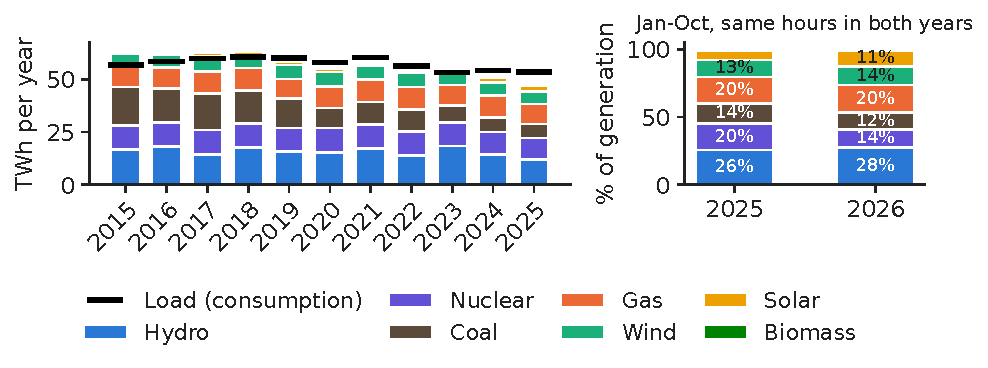
\includegraphics[width=\textwidth,height=0.547\textheight,keepaspectratio]{charts/en/mix_ro_annual.pdf}\end{center}\vspace{-3mm}
\chartsource{Source: energy-charts.info (Fraunhofer ISE); ENTSO-E (Transelectrica data for Romania). Data: 2015-2025 full years (left); Jan-Oct 2025 and 2026, hours reported in both years (right); cut-off 2026-10-31.}
\vspace{0.5mm}
\begin{itemize}\setlength{\itemsep}{0pt}
  \item Hydro = run-of-river (RoR) + reservoir, coal = lignite + hard coal
    \begin{itemize}\setlength{\itemsep}{0pt}
      \item Black bar = consumption, above the stack it means net imports
      \item Energy summed over reported hours (coverage $\ge$ 98.1\% in full years)
      \item Metered solar may miss rooftop output.
    \end{itemize}
\end{itemize}
\end{frame}

\begin{frame}{Romania: coal shrinks, solar grows, nuclear drops in 2026}
\framesubtitle{(Romania; energy-charts.info; data source: ENTSO-E)\hfill\tryit{notebook \S2}}
\small
\begin{center}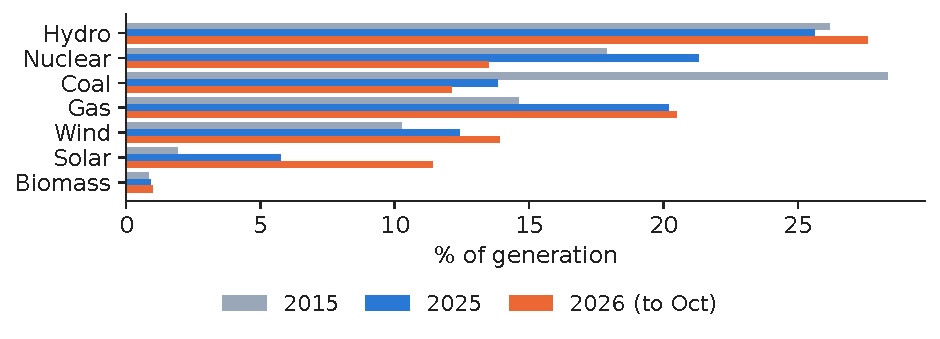
\includegraphics[width=\textwidth,height=0.409\textheight,keepaspectratio]{charts/en/mix_shares.pdf}\end{center}\vspace{-3mm}
\chartsource{Source: energy-charts.info (Fraunhofer ISE); ENTSO-E (Transelectrica data for Romania). Data: 2015, 2025 full years; Jan-Oct 2026, hours reported in both 2025 and 2026.}
\vspace{0.5mm}
\begin{itemize}\setlength{\itemsep}{0pt}
  \item Coal output: \ensuremath{-}63.9\% from 2015 to 2025
    \begin{itemize}\setlength{\itemsep}{0pt}
      \item Metered solar 2.2$\times$ over the same years.
    \end{itemize}
  \item Nuclear, Jan--Oct 2026 vs 2025: \ensuremath{-}31.3\% on hours reported in both years
    \begin{itemize}\setlength{\itemsep}{0pt}
      \item The true fall is at least as large, since the 29 unreported September days are left out.
    \end{itemize}
\end{itemize}
\par\vfill\manager{hydro producers and industrial consumers watch which plant becomes marginal when water or a reactor is missing.}\par\vspace{0.5mm}
\end{frame}

\begin{frame}{Where the course goes: seven lectures, one map of models}
\framesubtitle{(Weron, 2014, IJF; Ziel \& Weron, 2018, ENEECO)}
\footnotesize
\begin{columns}[T,onlytextwidth]
\begin{column}{0.56\textwidth}
\begin{block}{Course roadmap}
\begin{enumerate}\setlength{\itemsep}{0pt}\footnotesize
\item \textbf{Energy markets and their data} (today)
\item Forecasting: classical and expert autoregressive models with exogenous variables (ARX)
\item Volatility
\item Risk in energy companies: price--volume, cash flow at risk, imbalance, basis
\item Derivatives and hedging, including power purchase agreements
\item Renewables, storage, flexibility: cannibalisation, negative prices, batteries
\item Machine learning and foundation models for forecasting
\end{enumerate}
\end{block}
\end{column}
\begin{column}{0.41\textwidth}
\begin{itemize}\setlength{\itemsep}{1pt}
  \item \textbf{Model families}
    \begin{itemize}\setlength{\itemsep}{0pt}
      \item Fundamental: supply stack, fuel and carbon cost
      \item Reduced-form (mean reversion, jumps) and statistical
      \item Machine learning and hybrids
    \end{itemize}
  \item \textbf{Two views of the same data}
    \begin{itemize}\setlength{\itemsep}{0pt}
      \item Univariate: one long series of prices
      \item Multivariate: 24 (now 96) daily series, one per period
    \end{itemize}
  \item Every model must beat the \textbf{naive benchmark} of Section 3.
\end{itemize}
\end{column}
\end{columns}
\par\vfill\manager{ask any forecast vendor which family the model belongs to and by how much it beats the naive benchmark.}\par\vspace{0.5mm}
\end{frame}


\section{Energy data and stylized facts}

\subsection{Units, clocks and clean data}

\begin{frame}{Power and energy: a MW is not a MWh}
\framesubtitle{(energy-charts.info; World Bank Commodity Price Data)\hfill\tryit{notebook \S1}}
\footnotesize
\intuition{A megawatt (MW) is how fast energy flows; a megawatt-hour (MWh) is how much flowed, e.g.\ 1 MW for one hour.}
\begin{columns}[T,onlytextwidth]
\begin{column}{0.45\textwidth}
\[ E=\frac{1}{10^6}\sum_{t\ \text{reported}}\underbrace{P_t\,\Delta_t}_{\text{MWh}}\ [\text{TWh}] \]\[ \text{coverage}=\frac{\text{reported hours}}{\text{hours in the period}} \]{\footnotesize\begin{itemize}\setlength{\itemsep}{0pt}
  \item \textbf{\txtwhere}
    \begin{itemize}\setlength{\itemsep}{0pt}
      \item $P_t$ = mean power in interval $t$ (MW)
      \item $\Delta_t$ = its length (h)
      \item $E$ = energy in terawatt-hours (TWh), $1\ \text{TWh}=10^6\ \text{MWh}$.
    \end{itemize}
\end{itemize}\par}
\end{column}
\begin{column}{0.52\textwidth}
\begin{itemize}\setlength{\itemsep}{0pt}
  \item \textbf{On our data}: Romania consumed 53.56 TWh in 2025, a mean load of 6.1 gigawatts (GW).
  \item Missing hours are not filled, and every total comes with its coverage.
  \item \textbf{Reference prices}
    \begin{itemize}\setlength{\itemsep}{0pt}
      \item Base: mean of the delivery day
      \item Peak: mean of 08:00--20:00, Monday to Friday
    \end{itemize}
  \item Gas and oil are quoted in US dollars (USD) per million British thermal units (MMBtu) and per barrel (bbl)
    \begin{itemize}\setlength{\itemsep}{0pt}
      \item Conversion to EUR/MWh: Appendix G.
    \end{itemize}
\end{itemize}
\end{column}
\end{columns}
\par\vfill\manager{a 10 MW baseload contract delivers 240 MWh a day.}\par\vspace{0.5mm}
\end{frame}

\begin{frame}{One day of Romanian consumption: power in MW, energy in MWh}
\framesubtitle{(Romania; energy-charts.info; data source: ENTSO-E)\hfill\tryit{notebook \S1}}
\small
\begin{center}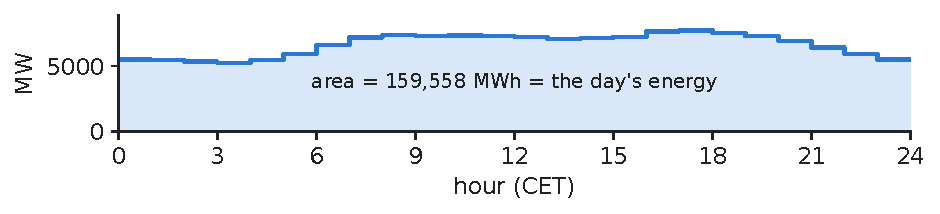
\includegraphics[width=\textwidth,height=0.353\textheight,keepaspectratio]{charts/en/day_load.pdf}\end{center}\vspace{-3mm}
\chartsource{Source: energy-charts.info (Fraunhofer ISE); ENTSO-E (Transelectrica data for Romania). Data: Romania, load on 2026-10-28 (CET day, 24 hourly values).}
\vspace{0.5mm}
\begin{itemize}\setlength{\itemsep}{0pt}
  \item \textbf{The curve} shows power: how much the country draws at each hour (MW)
    \begin{itemize}\setlength{\itemsep}{0pt}
      \item Minimum 5\,253 MW at 3:00, maximum 7\,719 MW at 17:00 (CET)
    \end{itemize}
  \item \textbf{The shaded area} is energy: 159\,558 MWh on 28 Oct 2026
    \begin{itemize}\setlength{\itemsep}{0pt}
      \item 24 hours $\times$ a mean of 6\,648 MW
    \end{itemize}
\end{itemize}
\par\vfill\manager{a supplier buys energy (MWh) for each interval
    \begin{itemize}\setlength{\itemsep}{0pt}
      \item The grid must cover the peak power (MW)
    \end{itemize}}\par\vspace{0.5mm}
\end{frame}

\begin{frame}{Clean data (1): delivery day, clock changes, zone changes}
\framesubtitle{(Lago, Marcjasz, De Schutter \& Weron, 2021, APEN)\hfill\tryit{notebook \S1}}
\footnotesize
\begin{itemize}\setlength{\itemsep}{1pt}
  \item \textbf{Clocks}: raw time stamps are in Coordinated Universal Time (UTC)
    \begin{itemize}\setlength{\itemsep}{0pt}
      \item Daily statistics use the SDAC delivery day, in Central European Time (CET) or, in summer, Central European Summer Time (CEST)
      \item A UTC day would put one or two hours into the wrong day.
    \end{itemize}
  \item \textbf{Clock changes}: the last Sunday of March has 23 hours, the last Sunday of October 25
    \begin{itemize}\setlength{\itemsep}{0pt}
      \item Daily means use the intervals that exist.
    \end{itemize}
  \item \textbf{Zone change}: Germany--Austria--Luxembourg was one zone until 30 Sep 2018
    \begin{itemize}\setlength{\itemsep}{0pt}
      \item Our series is spliced there.
    \end{itemize}
  \item Every chart and number is reproduced in the student notebook (notebooks/L1\_notebook.ipynb)
    \begin{itemize}\setlength{\itemsep}{0pt}
      \item One simulated figure, clearly labelled, illustrates white noise and the random walk.
    \end{itemize}
\end{itemize}
\end{frame}

\begin{frame}{Clean data (2): missing days and series breaks}
\framesubtitle{(Lago, Marcjasz, De Schutter \& Weron, 2021, APEN)\hfill\tryit{notebook \S1}}
\footnotesize
\begin{itemize}\setlength{\itemsep}{1pt}
  \item \textbf{Missing days}: the source (energy-charts.info, which republishes the prices of OPCOM and of the Independent Bulgarian Energy Exchange (IBEX) reported to ENTSO-E) has no price for some days, and gives no reason
    \begin{itemize}\setlength{\itemsep}{0pt}
      \item Romania: 5 days (21 Sep 2015, 20 Dec 2015, 21 Dec 2015, 31 Dec 2017, 17 Aug 2018)
      \item Bulgaria: the series starts 31 Oct 2016, although IBEX has run its day-ahead market since 19 Jan 2016, and 15 more days are missing up to 31 Dec 2016
      \item We do not fill these days, and no daily change is computed across a gap.
    \end{itemize}
  \item \textbf{Futures rolls}: the Brent front-month series jumps when the contract rolls
    \begin{itemize}\setlength{\itemsep}{0pt}
      \item Those days are dropped from return statistics.
    \end{itemize}
\end{itemize}
\par\vfill\manager{most forecasting errors at a supplier start in data handling (wrong clock, filled gaps), not in the model.}\par\vspace{0.5mm}
\end{frame}

\subsection{Price level and seasonality}

\begin{frame}{Prices jumped in 2021--2022 and never returned to the old level}
\framesubtitle{(energy-charts.info; prices: OPCOM, IBEX, HUPX, EPEX SPOT)\hfill\tryit{notebook \S3}}
\small
\begin{center}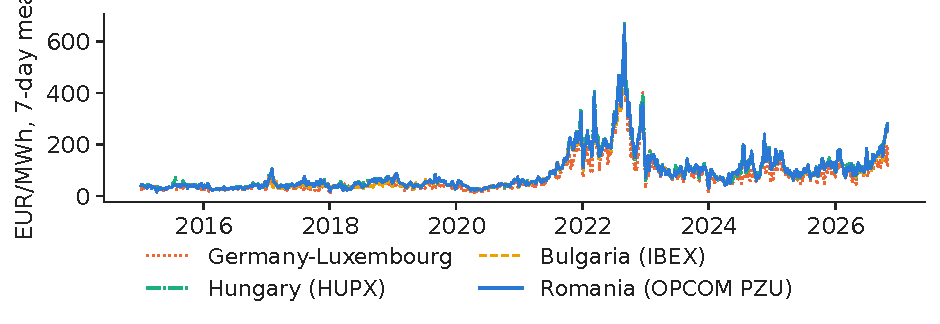
\includegraphics[width=\textwidth,height=0.534\textheight,keepaspectratio]{charts/en/prices_daily_4zones.pdf}\end{center}\vspace{-3mm}
\chartsource{Source: energy-charts.info (Fraunhofer ISE); prices from the exchanges OPCOM (RO), IBEX (BG), HUPX (HU), EPEX SPOT (DE-LU), via ENTSO-E. Data: 2015-01-01 to 2026-10-31 (BG from 2016-10-31).}
\vspace{0.5mm}
\begin{itemize}\setlength{\itemsep}{0pt}
  \item Romanian daily maximum 738.28 EUR/MWh on 30 Aug 2022
    \begin{itemize}\setlength{\itemsep}{0pt}
      \item RO, BG and HU move together (coupled), while Germany has been cheaper since 2023.
    \end{itemize}
\end{itemize}
\par\vfill\manager{an industrial consumer budgeting with pre-2021 prices is off by a factor of two to three.}\par\vspace{0.5mm}
\end{frame}

\begin{frame}{Volatility moves with the price level}
\framesubtitle{(energy-charts.info; own computation)}
\small
{\footnotesize\renewcommand{\arraystretch}{1.12}\setlength{\tabcolsep}{4pt}
\begin{tabular}{@{}lrrrrrrrrr@{}}\toprule
Mean, EUR/MWh & 2018 & 2019 & 2020 & 2021 & 2022 & 2023 & 2024 & 2025 & 2026 YTD \\ \midrule
RO & \cellcolor{Forest!52}46.4 & \cellcolor{Forest!50}50.4 & \cellcolor{Forest!55}39.5 & \cellcolor{Forest!20}111.4 & \cellcolor{Crimson!55}265.3 & \cellcolor{Forest!24}103.7 & \cellcolor{Forest!24}103.5 & \cellcolor{Forest!22}108.2 & \cellcolor{Forest!7}137.4 \\
BG & \cellcolor{Forest!55}39.9 & \cellcolor{Forest!51}47.5 & \cellcolor{Forest!55}39.3 & \cellcolor{Forest!19}108.7 & \cellcolor{Crimson!55}252.8 & \cellcolor{Forest!22}103.8 & \cellcolor{Forest!22}102.5 & \cellcolor{Forest!20}106.9 & \cellcolor{Forest!8}129.9 \\
HU & \cellcolor{Forest!49}51.0 & \cellcolor{Forest!50}50.4 & \cellcolor{Forest!55}39.0 & \cellcolor{Forest!20}113.8 & \cellcolor{Crimson!55}271.7 & \cellcolor{Forest!23}106.8 & \cellcolor{Forest!26}100.8 & \cellcolor{Forest!22}108.5 & \cellcolor{Forest!7}141.0 \\
DE-LU & \cellcolor{Forest!47}44.5 & \cellcolor{Forest!51}37.7 & \cellcolor{Forest!55}30.5 & \cellcolor{Forest!19}96.8 & \cellcolor{Crimson!55}235.5 & \cellcolor{Forest!20}95.2 & \cellcolor{Forest!29}78.5 & \cellcolor{Forest!23}89.3 & \cellcolor{Forest!10}114.0 \\
\multicolumn{10}{@{}l}{\textit{Volatility: standard deviation of daily price changes}} \\
RO & \cellcolor{Forest!50}10.9 & \cellcolor{Forest!49}11.5 & \cellcolor{Forest!55}8.6 & \cellcolor{Forest!19}25.2 & \cellcolor{Crimson!55}58.9 & \cellcolor{Forest!16}26.3 & \cellcolor{Forest!3}32.4 & \cellcolor{Forest!20}24.4 & \cellcolor{Forest!5}31.6 \\
BG & \cellcolor{Forest!46}13.6 & \cellcolor{Forest!48}12.8 & \cellcolor{Forest!55}9.8 & \cellcolor{Forest!23}23.6 & \cellcolor{Crimson!55}56.6 & \cellcolor{Forest!16}26.2 & \cellcolor{Forest!4}31.5 & \cellcolor{Forest!22}23.9 & \cellcolor{Forest!12}28.2 \\
HU & \cellcolor{Forest!53}9.2 & \cellcolor{Forest!53}9.2 & \cellcolor{Forest!55}8.5 & \cellcolor{Forest!18}24.8 & \cellcolor{Crimson!55}56.6 & \cellcolor{Forest!17}25.0 & \cellcolor{Crimson!5}34.7 & \cellcolor{Forest!17}25.3 & 32.6 \\
DE-LU & \cellcolor{Forest!55}11.5 & \cellcolor{Forest!54}11.9 & \cellcolor{Forest!55}11.5 & \cellcolor{Forest!8}34.4 & \cellcolor{Crimson!55}65.3 & \cellcolor{Forest!17}30.3 & \cellcolor{Forest!14}31.4 & \cellcolor{Forest!21}28.3 & \cellcolor{Forest!5}36.0 \\
\bottomrule\end{tabular}}
\par\vspace{0.5mm}{\scriptsize \begin{itemize}\setlength{\itemsep}{0pt}
  \item Colour within each row: green = lowest, red = highest (2026 YTD = Jan--Oct).
\end{itemize}}
\vspace{1mm}
\begin{itemize}\setlength{\itemsep}{1pt}
  \item 2026 YTD: Romania 137.45 vs 105.88 EUR/MWh in Jan--Oct 2025 (\ensuremath{+}29.8\%).
\end{itemize}
\par\vfill\manager{collateral for PZU purchases must scale with the price, since a 200 EUR/MWh market moves far more than a 50 one.}\par\vspace{0.5mm}
\end{frame}

\begin{frame}{Solar moved the cheapest hour of the day to midday}
\framesubtitle{(energy-charts.info; hourly day-ahead prices)\hfill\tryit{notebook \S3}}
\small
\begin{center}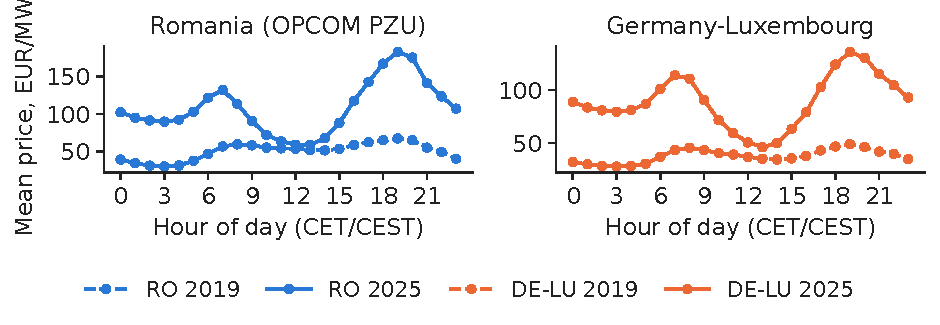
\includegraphics[width=\textwidth,height=0.493\textheight,keepaspectratio]{charts/en/profile_intraday.pdf}\end{center}\vspace{-3mm}
\chartsource{Source: energy-charts.info (Fraunhofer ISE); prices from the exchanges OPCOM (RO), IBEX (BG), HUPX (HU), EPEX SPOT (DE-LU), via ENTSO-E. Data: calendar years 2019 and 2025, hourly.}
\vspace{0.5mm}
\begin{itemize}\setlength{\itemsep}{0pt}
  \item From 2019 to 2025 the cheapest hour moved from night to midday
    \begin{itemize}\setlength{\itemsep}{0pt}
      \item 2025: cheapest at 13:00 (58.8 EUR/MWh in Romania), evening peak 182.5
      \item Evening/midday ratio 1.30 $\to$ 3.11, the ``duck curve''.
    \end{itemize}
\end{itemize}
\par\vfill\manager{a battery developer's revenue is this midday-to-evening spread, captured once or twice a day.}\par\vspace{0.5mm}
\end{frame}

\begin{frame}{Weekends are cheaper}
\framesubtitle{\hfill\tryit{notebook \S3}}
\footnotesize
\intuition{Factories and offices consume less on weekends, so fewer plants are needed and the price drops.}
\begin{columns}[T,onlytextwidth]
\begin{column}{0.50\textwidth}
\[ \hat s_j=\frac1W\sum_{w=1}^{W}\Big(\underbrace{p_{w,j}}_{\text{day }j\text{ of week }w}-\underbrace{\tfrac17\textstyle\sum_{i=1}^{7}p_{w,i}}_{\text{mean of week }w}\Big) \]{\footnotesize\begin{itemize}\setlength{\itemsep}{0pt}
  \item \textbf{\txtwhere}
    \begin{itemize}\setlength{\itemsep}{0pt}
      \item $j$ = weekday
      \item $W$ = number of complete weeks
      \item $\hat s_j$ = average distance of weekday $j$ from its own week's mean (EUR/MWh)
      \item Subtracting each week's mean removes level shifts such as 2022.
    \end{itemize}
\end{itemize}\par}
\end{column}
\begin{column}{0.47\textwidth}
\begin{itemize}\setlength{\itemsep}{1pt}
  \item \textbf{On our data}: 199 weeks, 2 Jan 2023 -- 25 Oct 2026.
\end{itemize}\vspace{0.5mm}{\scriptsize\renewcommand{\arraystretch}{1.05}\setlength{\tabcolsep}{4pt}
\begin{tabular}{@{}lrrrrrrr@{}}\toprule
 & Mon & Tue & Wed & Thu & Fri & Sat & Sun \\ \midrule
RO & \cellcolor{Crimson!46}9.1 & \cellcolor{Crimson!55}12.7 & \cellcolor{Crimson!55}12.6 & \cellcolor{Crimson!49}10.4 & \cellcolor{Crimson!31}3.4 & \cellcolor{Forest!22}\ensuremath{-}17.5 & \cellcolor{Forest!55}\ensuremath{-}30.7 \\
DE-LU & \cellcolor{Crimson!41}7.0 & \cellcolor{Crimson!53}11.0 & \cellcolor{Crimson!55}11.6 & \cellcolor{Crimson!44}7.9 & \cellcolor{Crimson!30}3.3 & \cellcolor{Forest!27}\ensuremath{-}15.8 & \cellcolor{Forest!55}\ensuremath{-}25.1 \\
\bottomrule\end{tabular}}\par\vspace{1mm}\begin{itemize}\setlength{\itemsep}{1pt}
  \item Sunday in Romania: $\hat s_{\text{Sun}}=$ \ensuremath{-}30.7 EUR/MWh relative to its week's mean.
\end{itemize}
\end{column}
\end{columns}
\par\vfill\manager{an industrial consumer can move flexible load (maintenance, pumping, charging) to Sunday and save that difference.}\par\vspace{0.5mm}
\end{frame}

\begin{frame}{Spring is cheap: water and sun meet mild demand}
\framesubtitle{(energy-charts.info; monthly means 2016--2025)\hfill\tryit{notebook \S3}}
\small
\begin{center}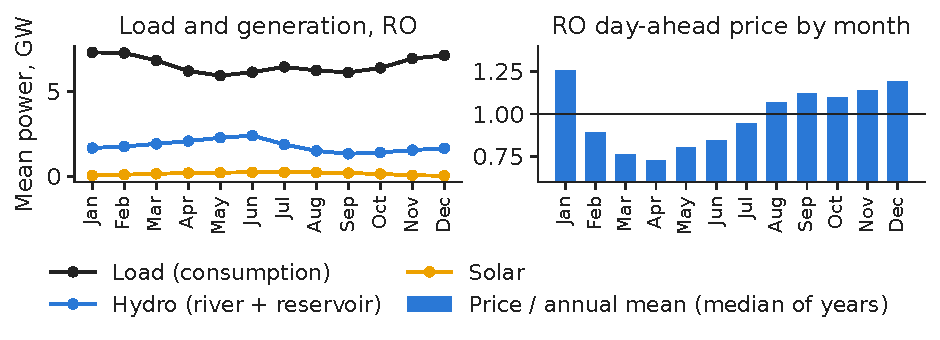
\includegraphics[width=\textwidth,height=0.415\textheight,keepaspectratio]{charts/en/profile_annual.pdf}\end{center}\vspace{-3mm}
\chartsource{Source: energy-charts.info (Fraunhofer ISE); prices from the exchanges OPCOM (RO), IBEX (BG), HUPX (HU), EPEX SPOT (DE-LU), via ENTSO-E. Data: monthly means 2016-2025.}
\vspace{0.5mm}
\begin{itemize}\setlength{\itemsep}{0pt}
  \item Price relative to the annual mean: highest in January (1.26), lowest in April (0.72)
    \begin{itemize}\setlength{\itemsep}{0pt}
      \item Consumption is highest in January--February and lowest in May
      \item Hydro peaks in June (snow melt).
    \end{itemize}
\end{itemize}
\par\vfill\manager{a hydro producer saves reservoir water in spring, when power is cheap, to sell it in winter and late summer.}\par\vspace{0.5mm}
\end{frame}

\subsection{Spikes and negative prices}

\begin{frame}{Spikes: a few hours with extreme prices}
\framesubtitle{(Janczura, Trück, Weron \& Wolff, 2013, ENEECO)\hfill\tryit{notebook \S4}}
\footnotesize
\intuition{A spike is an interval whose price is far above what is normal for that year.}
\begin{columns}[T,onlytextwidth]
\begin{column}{0.55\textwidth}
\[ p_t>\underbrace{Q_{3,y}}_{\text{75th percentile}}+3\cdot\underbrace{(Q_{3,y}-Q_{1,y})}_{\text{interquartile range (IQR)}} \]{\footnotesize\begin{itemize}\setlength{\itemsep}{0pt}
  \item \textbf{\txtwhere}
    \begin{itemize}\setlength{\itemsep}{0pt}
      \item $Q_{1,y},Q_{3,y}$ = 25th and 75th percentiles of all prices of year $y$, weighted by interval length (15-min intervals count a quarter)
      \item Percentiles are robust, so spikes barely move the threshold.
    \end{itemize}
\end{itemize}\par}
\end{column}
\begin{column}{0.42\textwidth}
{\scriptsize\renewcommand{\arraystretch}{1.0}\setlength{\tabcolsep}{4pt}
\begin{tabular}{@{}lrrr@{}}\toprule
Year & RO thr. & RO h & DE-LU h \\ \midrule
2020 & 109 & \cellcolor{MainBlue!12}54.00 & \cellcolor{MainBlue!6}30.00 \\
2021 & 394 & \cellcolor{MainBlue!15}69.00 & \cellcolor{MainBlue!60}\textcolor{white}{280.00} \\
2022 & 873 & \cellcolor{MainBlue!1}4.00 & \cellcolor{MainBlue!1}4.00 \\
2023 & 292 & \cellcolor{MainBlue!8}38.00 & \cellcolor{MainBlue!3}13.00 \\
2024 & 274 & \cellcolor{MainBlue!59}\textcolor{white}{276.00} & \cellcolor{MainBlue!15}72.00 \\
2025 & 285 & \cellcolor{MainBlue!26}120.00 & \cellcolor{MainBlue!19}88.75 \\
2026 & 427 & \cellcolor{MainBlue!8}39.25 & \cellcolor{MainBlue!7}32.25 \\
\bottomrule\end{tabular}}\par\vspace{1mm}\begin{itemize}\setlength{\itemsep}{1pt}
  \item Highest Romanian price in our data: 1021.61 EUR/MWh on 3 Sep 2024, 19:00 CEST.
\end{itemize}
\end{column}
\end{columns}
\par\vfill\manager{a supplier with fixed-price retail contracts loses most of the year's margin in a few dozen spike hours, which is why it hedges.}\par\vspace{0.5mm}
\end{frame}

\begin{frame}{Negative prices reached Romania in 2023 and are now routine}
\framesubtitle{(energy-charts.info; own count, a 15-min MTU = 0.25 h)\hfill\tryit{notebook \S4}}
\small
\begin{center}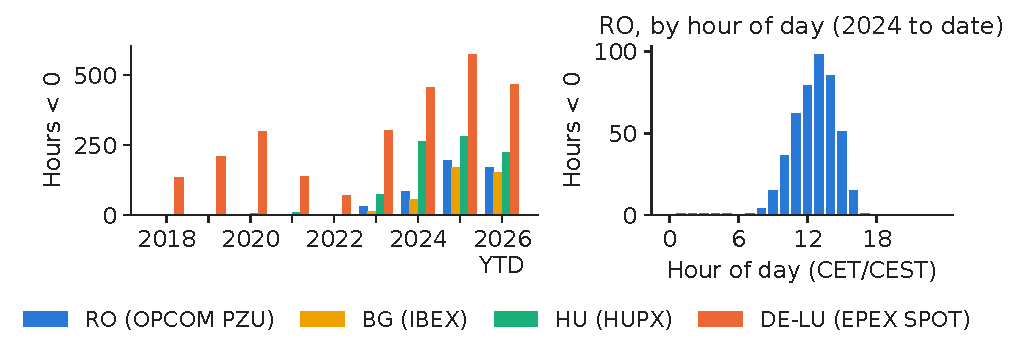
\includegraphics[width=\textwidth,height=0.491\textheight,keepaspectratio]{charts/en/negative_prices.pdf}\end{center}\vspace{-3mm}
\chartsource{Source: energy-charts.info (Fraunhofer ISE); prices from the exchanges OPCOM (RO), IBEX (BG), HUPX (HU), EPEX SPOT (DE-LU), via ENTSO-E. Data: 2018 to 2026-10-31; a 15-min MTU counts 0.25 h.}
\vspace{0.5mm}
\begin{itemize}\setlength{\itemsep}{0pt}
  \item First negative Romanian price: 21 May 2023
    \begin{itemize}\setlength{\itemsep}{0pt}
      \item Since 2024, 91.1\% of negative hours fall between 10:00 and 16:00 and 83.9\% on weekends
      \item Bars in hour-equivalents.
    \end{itemize}
\end{itemize}
\par\vfill\manager{a solar park without storage sells much of its output in the cheapest hours of the year (Lecture 6).}\par\vspace{0.5mm}
\end{frame}

\begin{frame}{Counting negative prices correctly: hour-equivalents}
\framesubtitle{(energy-charts.info; own computation)\hfill\tryit{notebook \S4}}
\small
{\footnotesize\renewcommand{\arraystretch}{1.2}\setlength{\tabcolsep}{4pt}
\begin{tabular}{@{}lrrrrrrr@{}}\toprule
Zone & 2022 & 2023 & 2024 & 2025 & 2026 YTD & Jan--Oct 2025 & 2026: 15-min MTUs \\ \midrule
RO & 0 & \cellcolor{MainBlue!3}32 & \cellcolor{MainBlue!9}85 & \cellcolor{MainBlue!20}196 & \cellcolor{MainBlue!18}171.75 & 196 & 687 \\
BG & 0 & \cellcolor{MainBlue!1}11 & \cellcolor{MainBlue!6}55 & \cellcolor{MainBlue!18}170 & \cellcolor{MainBlue!16}152.25 & 170 & 609 \\
HU & 0 & \cellcolor{MainBlue!8}74 & \cellcolor{MainBlue!27}262 & \cellcolor{MainBlue!29}281 & \cellcolor{MainBlue!23}223.50 & 281 & 894 \\
DE-LU & \cellcolor{MainBlue!7}69 & \cellcolor{MainBlue!31}301 & \cellcolor{MainBlue!48}\textcolor{white}{457} & \cellcolor{MainBlue!60}\textcolor{white}{574.75} & \cellcolor{MainBlue!49}\textcolor{white}{465} & 574.75 & 1\,860 \\
\bottomrule\end{tabular}}
\par\vspace{0.5mm}{\scriptsize \begin{itemize}\setlength{\itemsep}{0pt}
  \item Hours with a negative day-ahead price; darker = more hours; last column: negative quarter-hours (= 4 $\times$ hour-equivalents).
\end{itemize}}
\vspace{1.5mm}
\begin{itemize}\setlength{\itemsep}{0pt}
  \item Romania had none before 2023
    \begin{itemize}\setlength{\itemsep}{0pt}
      \item Germany had them every year (inflexible plants plus wind).
    \end{itemize}
  \item RO, BG and HU move together (coupled), but Hungary has had more negative hours since 2023.
  \item Jan--Oct 2026: Romania 171.75 h vs 196.00 h a year earlier
    \begin{itemize}\setlength{\itemsep}{0pt}
      \item Growth is not automatic (Case study d).
    \end{itemize}
\end{itemize}
\par\vfill\manager{in reports to the board, write ``687 quarter-hours (171.75 h)''
    \begin{itemize}\setlength{\itemsep}{0pt}
      \item Never a bare number.
    \end{itemize}}\par\vspace{0.5mm}
\end{frame}

\subsection{Distribution and volatility}

\begin{frame}{Prices can be zero or negative: use differences or asinh}
\framesubtitle{(Uniejewski, Weron \& Ziel, 2018, IEEE TPWRS)\hfill\tryit{notebook \S5}}
\small
\intuition{Percentage changes need a positive price; a transformation that accepts any sign keeps the zero and negative hours.}
\vspace{-1mm}\[ y_t=\operatorname{asinh}(x_t)=\ln\big(x_t+\sqrt{x_t^2+1}\big),\quad x_t=\frac{p_t-\tilde p}{\widehat{\mathrm{MAD}}},\quad \operatorname{asinh}(x)\approx\operatorname{sign}(x)\ln(2|x|)\ \text{for large } |x| \]\vspace{-2mm}
\begin{center}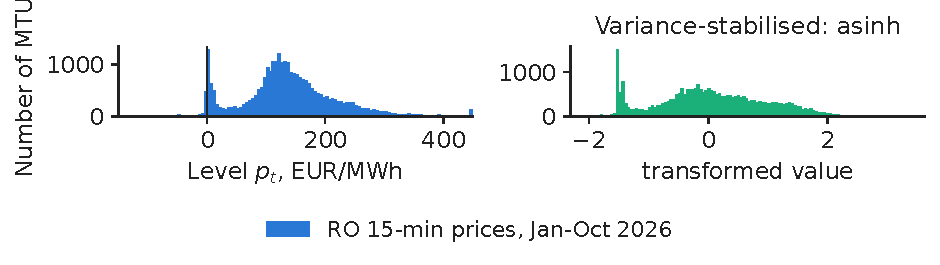
\includegraphics[width=\textwidth,height=0.276\textheight,keepaspectratio]{charts/en/asinh_ro.pdf}\end{center}\vspace{-3mm}
\chartsource{Source: energy-charts.info (Fraunhofer ISE); prices from the exchanges OPCOM (RO), IBEX (BG), HUPX (HU), EPEX SPOT (DE-LU), via ENTSO-E. Data: all 15-min MTUs, 2026-01-01 to 2026-10-31.}
\vspace{0.5mm}
\begin{itemize}\setlength{\itemsep}{0pt}
  \item $\tilde p$ = median, $\widehat{\mathrm{MAD}}$ = median absolute deviation (MAD) $\times1.4826$
    \begin{itemize}\setlength{\itemsep}{0pt}
      \item Report PZU moves in EUR/MWh.
    \end{itemize}
  \item Jan--Oct 2026: 1\,189 of 29\,184 quarter-hours $\le 0$ (502 exactly 0)
    \begin{itemize}\setlength{\itemsep}{0pt}
      \item Skewness 1.19 $\to$ 0.13
      \item Excess kurtosis 6.73 $\to$ \ensuremath{-}0.55.
    \end{itemize}
\end{itemize}
\end{frame}

\begin{frame}{Extreme oil moves are far more frequent than a normal curve allows}
\framesubtitle{(Jarque \& Bera, 1980, Econ.\ Letters; Yahoo Finance BZ=F)\hfill\tryit{notebook \S5}}
\small
\intuition{``Fat tails'': very large up or down days happen much more often than a bell curve would allow.}
\begin{center}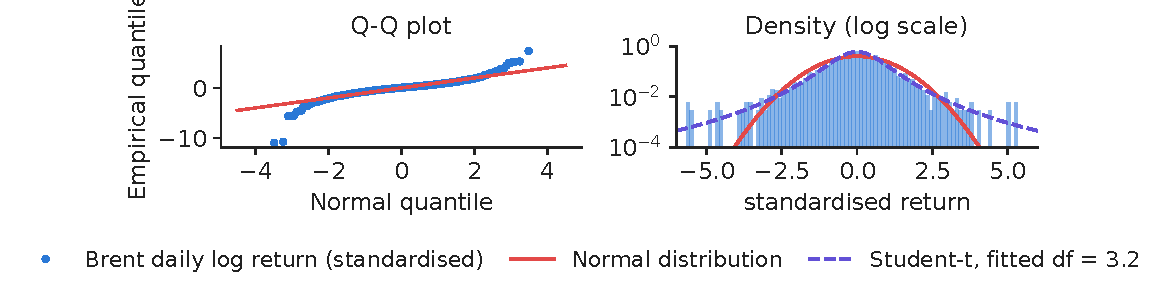
\includegraphics[width=\textwidth,height=0.396\textheight,keepaspectratio]{charts/en/tails_brent.pdf}\end{center}\vspace{-3mm}
\chartsource{Source: Yahoo Finance (BZ=F). Data: 2015-01-05 to 2026-10-30.}
\vspace{0.5mm}
\begin{itemize}\setlength{\itemsep}{0pt}
  \item Brent daily log returns, 5 Jan 2015 -- 30 Oct 2026, without the 141 contract-roll days
    \begin{itemize}\setlength{\itemsep}{0pt}
      \item Moves beyond 4 standard deviations: 16 observed vs 0.18 expected under normality
      \item Excess kurtosis 13.98 (formulas and the Jarque--Bera (JB) test: Appendix F).
    \end{itemize}
\end{itemize}
\par\vfill\manager{a fuel-budget limit built on the normal curve understates how often a crisis day comes (Lecture 4).}\par\vspace{0.5mm}
\end{frame}

\begin{frame}{Calm and turbulent periods come in clusters}
\framesubtitle{(Ljung \& Box, 1978, Biometrika)\hfill\tryit{notebook \S5}}
\small
\intuition{A big move today makes another big move tomorrow more likely, even if its direction is unpredictable.}
\vspace{-1mm}\[ Q(m)=T(T+2)\sum_{k=1}^{m}\frac{\hat\rho_k^2}{T-k}\ \sim\ \chi^2_m\quad\text{(Ljung--Box)} \]\vspace{-2mm}
\begin{center}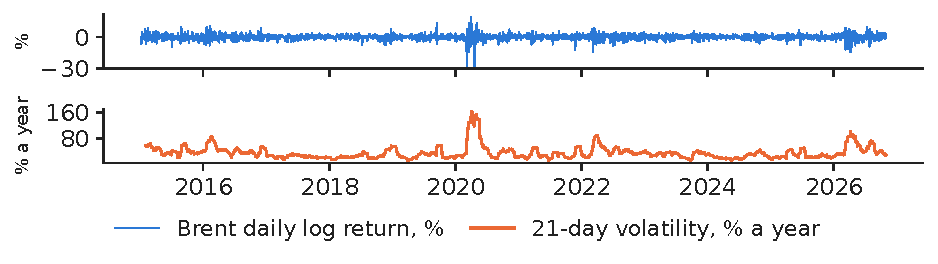
\includegraphics[width=\textwidth,height=0.329\textheight,keepaspectratio]{charts/en/volclust_brent.pdf}\end{center}\vspace{-3mm}
\chartsource{Source: Yahoo Finance (BZ=F). Data: 2015-01-05 to 2026-10-30.}
\vspace{0.5mm}
\begin{itemize}\setlength{\itemsep}{0pt}
  \item Brent: $Q_{10}(r)=$ 28.1 but $Q_{10}(r^2)=$ 506.9 (5\% critical value 18.31)
    \begin{itemize}\setlength{\itemsep}{0pt}
      \item Little memory in the direction of moves, a lot in their size.
    \end{itemize}
\end{itemize}
\par\vfill\manager{after a shock, a risk desk keeps wider limits for weeks, not days (Lecture 3).}\par\vspace{0.5mm}
\end{frame}


\section{Time-series toolkit}

\subsection{Stationarity and autocorrelation}

\begin{frame}{Stationary means the rules of the game do not change over time}
\framesubtitle{(Hyndman \& Athanasopoulos, 2021, OTexts)\hfill\tryit{notebook \S6}}
\small
\intuition{A series is (weakly) stationary if its average, its spread and its memory are the same in every period; memory depends only on the lag $k$, not on the date $t$.}
\vspace{-1mm}\[ \E X_t=\mu,\quad \Var X_t=\gamma_0,\quad \Cov(X_t,X_{t-k})=\gamma_k\quad \text{for every } t \]\vspace{-2mm}
\begin{center}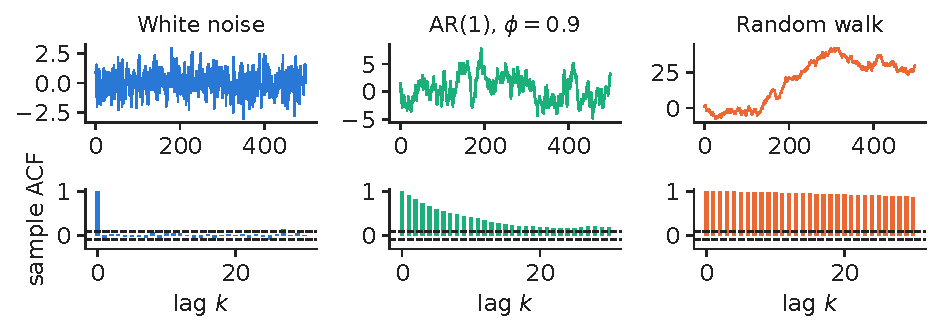
\includegraphics[width=\textwidth,height=0.243\textheight,keepaspectratio]{charts/en/sim_wn_ar_rw.pdf}\end{center}\vspace{-3mm}
\chartsource{\simlabel\ Source: simulation, numpy, seed 20261104. Data: T = 500, N(0,1) shocks.}
\vspace{0.5mm}
\begin{itemize}\setlength{\itemsep}{0pt}
  \item Three simulated series: white noise, a first-order autoregressive (AR) model AR(1) with $\phi=0.9$, which reverts to its mean, and a random walk, whose shocks are permanent.
  \item A random walk has a level autocorrelation close to 1 (here 0.96 at lag 10), not a low one.
\end{itemize}
\par\vfill\manager{a historical average price is a forecast only if the series is stationary
    \begin{itemize}\setlength{\itemsep}{0pt}
      \item Test it before budgeting with it.
    \end{itemize}}\par\vspace{0.5mm}
\end{frame}

\begin{frame}{Autocorrelation measures how much today's price remembers the past}
\framesubtitle{(Hyndman \& Athanasopoulos, 2021; Ljung \& Box, 1978)\hfill\tryit{notebook \S6}}
\footnotesize
\intuition{The autocorrelation at lag $k$ is the correlation between the series and itself shifted by $k$ periods.}
\begin{columns}[T,onlytextwidth]
\begin{column}{0.52\textwidth}
\[ \hat\rho_k=\frac{\sum_{t=k+1}^{T}(x_t-\bar x)(x_{t-k}-\bar x)}{\sum_{t=1}^{T}(x_t-\bar x)^2} \]\begin{itemize}\setlength{\itemsep}{1pt}
  \item White-noise band: $\pm1.96/\sqrt T$.
  \item Bartlett band at lag $k$: $\pm1.96\sqrt{(1+2\sum_{j<k}\hat\rho_j^2)/T}$, valid if the true autocorrelation is zero beyond lag $k-1$.
  \item Partial autocorrelation function (PACF): memory at lag $k$ net of shorter lags.
\end{itemize}
\end{column}
\begin{column}{0.45\textwidth}
\begin{itemize}\setlength{\itemsep}{1pt}
  \item \textbf{Four reading rules}
    \begin{itemize}\setlength{\itemsep}{0pt}
      \item Slow decay from near 1: persistence or a unit root; test it
      \item Geometric decay, PACF cut after $p$ lags: an AR($p$) model
      \item Peaks at lags 7, 14 (days) or 24, 168 (hours): seasonality
      \item All inside the band: no linear memory (check $x_t^2$ too)
    \end{itemize}
\end{itemize}
\end{column}
\end{columns}
\par\vfill\manager{a supplier's forecast for tomorrow starts from ``same weekday last week'': $\hat\rho_7=$ 0.672 in Romania since 2023.}\par\vspace{0.5mm}
\end{frame}

\begin{frame}{Prices remember yesterday, last week and the same hour}
\framesubtitle{(Ziel \& Weron, 2018, ENEECO)\hfill\tryit{notebook \S6}}
\small
\begin{center}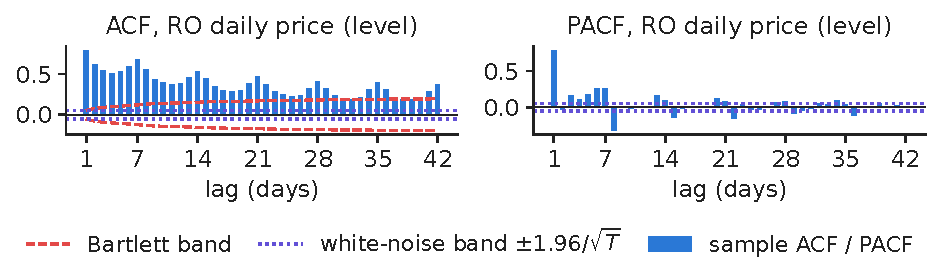
\includegraphics[width=\textwidth,height=0.330\textheight,keepaspectratio]{charts/en/acf_pacf_ro_daily.pdf}\end{center}\vspace{-3mm}
\chartsource{Source: energy-charts.info (Fraunhofer ISE); prices from the exchanges OPCOM (RO), IBEX (BG), HUPX (HU), EPEX SPOT (DE-LU), via ENTSO-E. Data: 2023-01-01 to 2026-10-31, T = 1400.}
\begin{center}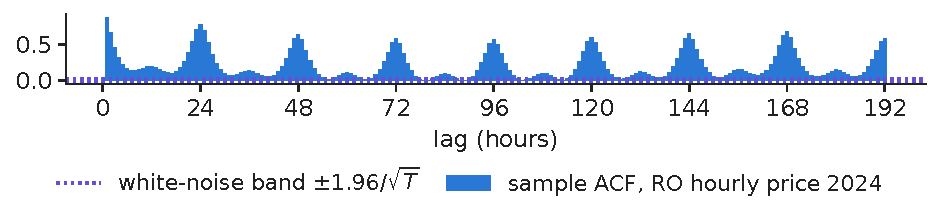
\includegraphics[width=\textwidth,height=0.230\textheight,keepaspectratio]{charts/en/acf_ro_hourly.pdf}\end{center}\vspace{-3mm}
\chartsource{Source: energy-charts.info (Fraunhofer ISE); prices from the exchanges OPCOM (RO), IBEX (BG), HUPX (HU), EPEX SPOT (DE-LU), via ENTSO-E. Data: 2024, hourly, T = 8784.}
\begin{itemize}\setlength{\itemsep}{1pt}
  \item Daily, 1 Jan 2023 -- 31 Oct 2026: $\hat\rho_1=$ 0.789, $\hat\rho_7=$ 0.672, PACF $\hat\alpha_7=$ 0.257
    \begin{itemize}\setlength{\itemsep}{0pt}
      \item Hourly, 2024: $\hat\rho_{24}=$ 0.776, $\hat\rho_{168}=$ 0.681.
    \end{itemize}
\end{itemize}
\end{frame}

\begin{frame}{The benchmark to beat: the naive forecast}
\framesubtitle{(Nogales et al., 2002, IEEE TPWRS; Weron, 2014, IJF; Lago et al., 2021, APEN)\hfill\tryit{notebook \S6}}
\small
\intuition{Tomorrow's price for each hour is today's price for that hour --- after weekends, the same day last week.}
\vspace{-1mm}\[ \hat p_{d,h}=\begin{cases} p_{d-1,h} & d=\text{Tue--Fri}\\ p_{d-7,h} & d=\text{Mon, Sat, Sun}\end{cases},\qquad \mathrm{MAE}=\frac{1}{n}\sum_{d,h}|p_{d,h}-\hat p_{d,h}| \]\vspace{-2mm}
\begin{center}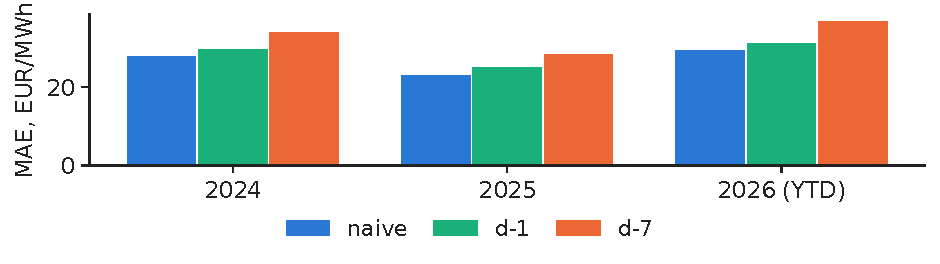
\includegraphics[width=\textwidth,height=0.247\textheight,keepaspectratio]{charts/en/naive_bar.pdf}\end{center}\vspace{-3mm}
\chartsource{Source: energy-charts.info (Fraunhofer ISE); prices from the exchanges OPCOM (RO), IBEX (BG), HUPX (HU), EPEX SPOT (DE-LU), via ENTSO-E. Data: hourly day-ahead prices, 2024-01 to 2026-10.}
\vspace{0.5mm}
\begin{itemize}\setlength{\itemsep}{0pt}
  \item Mean absolute error (MAE), EUR/MWh: Romania 2025, 22.9 at a mean price of 108.2
    \begin{itemize}\setlength{\itemsep}{0pt}
      \item The weekday/weekend rule beats both pure lags in 7 of 8 years
      \item All years and Germany: Appendix E.
    \end{itemize}
\end{itemize}
\par\vfill\manager{before paying for a forecasting service, ask for its MAE next to this benchmark.}\par\vspace{0.5mm}
\end{frame}

\subsection{Unit-root tests, decomposition, smoothing}

\begin{frame}{Do shocks die out or stay? Two tests ask it from opposite sides}
\framesubtitle{(Dickey \& Fuller, 1979, JASA; Kwiatkowski et al., 1992, J.\ Econometrics)\hfill\tryit{notebook \S7}}
\footnotesize
\intuition{One test starts from ``shocks are permanent'' and looks for a pull back to a mean; the other starts from ``the series is stable'' and looks for a slow drift.}
\begin{columns}[T,onlytextwidth]
\begin{column}{0.55\textwidth}
\[ \Delta x_t=\alpha+\underbrace{\gamma\,x_{t-1}}_{\text{pull to the mean}}+\underbrace{\textstyle\sum_{j}\delta_j\Delta x_{t-j}}_{\text{extra lags}}+u_t \]{\footnotesize\begin{itemize}\setlength{\itemsep}{0pt}
  \item \textbf{\txtwhere}
    \begin{itemize}\setlength{\itemsep}{0pt}
      \item Augmented Dickey--Fuller (ADF): $H_0:\gamma=0$ (unit root), $\hat\gamma/\mathrm{se}$ against Dickey--Fuller critical values (about $-2.86$ at 5\%), lags $p$ chosen by the Akaike information criterion (AIC)
      \item Kwiatkowski--Phillips--Schmidt--Shin (KPSS): $H_0$ = stationary, large values reject (0.463 at 5\%)
      \item Full formulas: Appendix A.
    \end{itemize}
\end{itemize}\par}
\end{column}
\begin{column}{0.42\textwidth}
{\scriptsize\renewcommand{\arraystretch}{1.05}\setlength{\tabcolsep}{4pt}
\begin{tabular}{@{}lll@{}}\toprule
 & KPSS: keep & KPSS: reject \\ \midrule
ADF: reject & \cellcolor{Forest!25}stationary & \cellcolor{Bitter!30}conflict \\
ADF: keep & inconclusive & \cellcolor{Crimson!25}unit root$^{*}$ \\
\bottomrule\end{tabular}}\par\vspace{1mm}\begin{itemize}\setlength{\itemsep}{1pt}
  \item $^{*}$Consistent with a unit root, not a proof: ADF has low power against slow mean reversion, and level breaks (2022) push it towards ``unit root''.
\end{itemize}
\end{column}
\end{columns}
\par\vfill\manager{if a supplier's price can carry permanent shocks, ``prices will come back to normal'' is not a safe budget assumption.}\par\vspace{0.5mm}
\end{frame}

\begin{frame}{One verdict per series: levels drift, changes are stable}
\framesubtitle{(own computation; constant only; ADF lags by AIC; 5\% level)\hfill\tryit{notebook \S7}}
\small
{\footnotesize\renewcommand{\arraystretch}{1.0}\setlength{\tabcolsep}{4pt}
\begin{tabular}{@{}llrrrrrl@{}}\toprule
Series & Sample & $T$ & ADF & $p$ & KPSS & $p$ & Verdict \\ \midrule
RO price, level & 2015--2026 & 4\,317 & \ensuremath{-}2.71 & 0.073 & 3.645 & $<$0.01 & \cellcolor{Crimson!25}unit root$^{*}$ \\
RO price, daily change & 2015--2026 & 4\,312 & \ensuremath{-}14.81 & $<$0.001 & 0.045 & $>$0.10 & \cellcolor{Forest!25}stationary \\
DE-LU price, level & 2015--2026 & 4\,322 & \ensuremath{-}3.54 & 0.007 & 3.441 & $<$0.01 & \cellcolor{Bitter!30}conflict \\
Brent, log price & 2015--2026 & 2\,976 & \ensuremath{-}2.19 & 0.212 & 3.820 & $<$0.01 & \cellcolor{Crimson!25}unit root$^{*}$ \\
Brent, log return & 2015--2026 & 2\,975 & \ensuremath{-}10.79 & $<$0.001 & 0.049 & $>$0.10 & \cellcolor{Forest!25}stationary \\
RO hydro, deseasonalised & 2015--2025 & 132 & \ensuremath{-}4.19 & $<$0.001 & 0.354 & 0.097 & \cellcolor{Forest!25}stationary \\
\bottomrule\end{tabular}}
\par\vspace{0.5mm}{\scriptsize \begin{itemize}\setlength{\itemsep}{0pt}
  \item $^{*}$Consistent with a unit root (not rejected); not a proof.
\end{itemize}}
\vspace{1mm}
\begin{itemize}\setlength{\itemsep}{1pt}
  \item Romanian and Brent \textbf{levels} are consistent with a unit root, while their \textbf{changes} are stationary.
  \item Germany: both tests reject (conflict): mean reversion plus the 2021--2022 level shift.
  \item Hydro is tested without its monthly means (a seasonal series)
    \begin{itemize}\setlength{\itemsep}{0pt}
      \item Romanian price since 2023 only: ADF $p=$ 0.361, KPSS 1.039.
    \end{itemize}
\end{itemize}
\par\vfill\manager{model price \emph{changes} (or transformed prices) and put seasonality in explicitly.}\par\vspace{0.5mm}
\end{frame}

\begin{frame}{Decomposition splits a series into trend, season and the rest}
\framesubtitle{(Cleveland et al., 1990, JOS; Hyndman \& Athanasopoulos, 2021)\hfill\tryit{notebook \S8}}
\small
\intuition{The classical method keeps the season fixed; Seasonal--Trend decomposition using Loess (STL) lets it evolve.}
\vspace{-1mm}\[ x_t=\underbrace{T_t}_{\text{trend}}+\underbrace{S_t}_{\text{season}}+\underbrace{R_t}_{\text{remainder}} \]\vspace{-2mm}
\begin{center}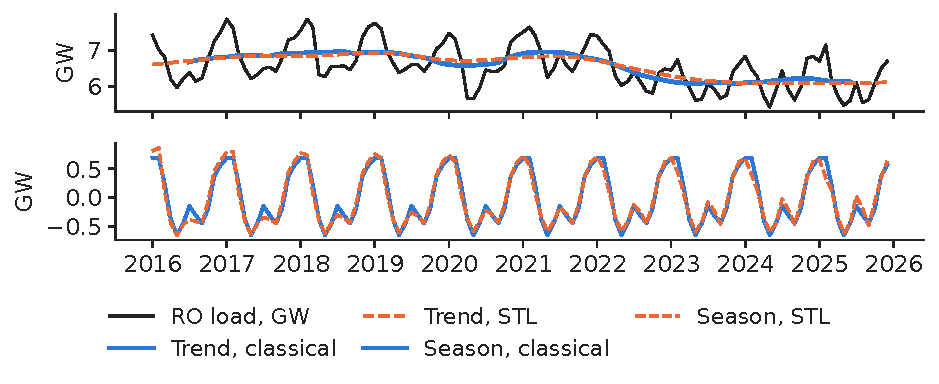
\includegraphics[width=\textwidth,height=0.234\textheight,keepaspectratio]{charts/en/decomp_load.pdf}\end{center}\vspace{-3mm}
\chartsource{Source: energy-charts.info (Fraunhofer ISE); ENTSO-E (Transelectrica data for Romania). Data: 2016-01 to 2025-12, monthly mean load.}
\vspace{0.5mm}
\begin{itemize}\setlength{\itemsep}{0pt}
  \item Romanian load vs trend: Jan \ensuremath{+}0.69, Feb \ensuremath{+}0.69, May \ensuremath{-}0.65 GW
    \begin{itemize}\setlength{\itemsep}{0pt}
      \item STL amplitude 1.52 $\to$ 1.27 GW
      \item Moving-average (MA) weights: Appendix B.
    \end{itemize}
\end{itemize}
\par\vfill\manager{Transelectrica and suppliers plan monthly capacity with seasonal indices
    \begin{itemize}\setlength{\itemsep}{0pt}
      \item STL shows when the pattern itself shifts.
    \end{itemize}}\par\vspace{0.5mm}
\end{frame}

\begin{frame}{Exponential smoothing: recent data count more}
\framesubtitle{(Hyndman \& Athanasopoulos, 2021, OTexts, ch.\ 8)\hfill\tryit{notebook \S9}}
\small
\intuition{The smoothed level is a weighted average of all past values, with weights shrinking geometrically into the past.}
\vspace{-1mm}\[ \ell_t=\underbrace{\alpha x_t}_{\text{news}}+\underbrace{(1-\alpha)\ell_{t-1}}_{\text{memory}},\qquad \alpha=1-2^{-1/h} \]\vspace{-2mm}
\begin{center}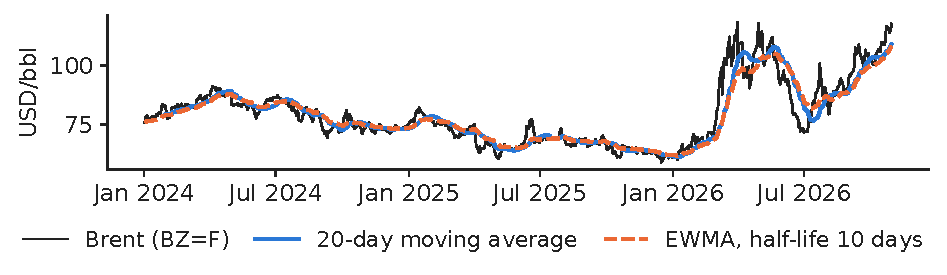
\includegraphics[width=\textwidth,height=0.237\textheight,keepaspectratio]{charts/en/smooth_brent.pdf}\end{center}\vspace{-3mm}
\chartsource{Source: Yahoo Finance (BZ=F). Data: 2024-01-02 to 2026-10-30.}
\vspace{0.5mm}
\begin{itemize}\setlength{\itemsep}{0pt}
  \item $h$ = half-life: after $h$ days an observation keeps half of its weight.
  \item Simple moving average (SMA) and exponentially weighted moving average (EWMA, $\alpha=$ 0.067)
    \begin{itemize}\setlength{\itemsep}{0pt}
      \item The best simple exponential smoothing (SES) weight is 0.948 $\approx1$, almost the last price.
    \end{itemize}
\end{itemize}
\par\vfill\manager{a fuel buyer can use an EWMA as a contract reference price
    \begin{itemize}\setlength{\itemsep}{0pt}
      \item As a forecast it adds little over the last price.
    \end{itemize}}\par\vspace{0.5mm}
\end{frame}


\section{Case studies on current data}

\subsection{(a) Wet 2023, dry 2025}

\begin{frame}{Case study (a): 2025 hydro output was a third below wet 2023}
\framesubtitle{(energy-charts.info; data source: ENTSO-E)\hfill\tryit{notebook \S10a}}
\small
\begin{center}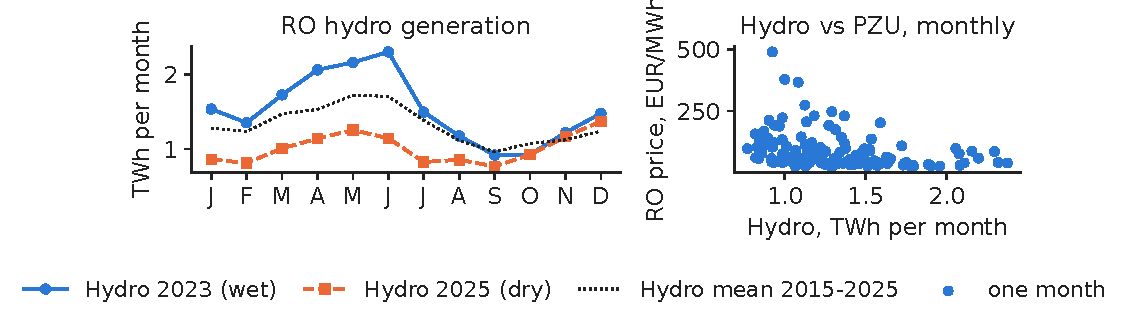
\includegraphics[width=\textwidth,height=0.419\textheight,keepaspectratio]{charts/en/hydro_case.pdf}\end{center}\vspace{-3mm}
\chartsource{Source: energy-charts.info (Fraunhofer ISE); ENTSO-E (Transelectrica data for Romania). Data: monthly, 2015-01 to 2025-12.}
\vspace{0.5mm}
\begin{itemize}\setlength{\itemsep}{0pt}
  \item Hydro (run-of-river + reservoir): 18.34 TWh in 2023 (highest since 2015) vs 12.15 TWh in 2025 (lowest), i.e.\ \textbf{\ensuremath{-}33.8\%}
    \begin{itemize}\setlength{\itemsep}{0pt}
      \item Against the 2015--2025 mean of 15.85 TWh: \ensuremath{-}23.3\%.
    \end{itemize}
  \item In the same years Romania went from net exporter (\ensuremath{-}3.06 TWh) to net importer (\ensuremath{+}3.76 TWh)
    \begin{itemize}\setlength{\itemsep}{0pt}
      \item Consistent with less water, but nuclear, demand and prices abroad also moved.
    \end{itemize}
\end{itemize}
\par\vfill\manager{a hydro producer's annual output and a net importer's bill depend on rain as much as on the market.}\par\vspace{0.5mm}
\end{frame}

\begin{frame}{Case study (a): wetter months go with lower Romanian prices}
\framesubtitle{(own estimation; Newey--West standard errors)\hfill\tryit{notebook \S10a}}
\footnotesize
\intuition{Holding the gas price fixed, months with more hydro output have had lower Romanian prices --- an association, not a measured effect.}
\begin{columns}[T,onlytextwidth]
\begin{column}{0.50\textwidth}
\[ p_m=\beta_0+\underbrace{\beta_1\,\mathrm{Hydro}_m}_{\text{water}}+\underbrace{\beta_2\,\mathrm{TTF}_m}_{\text{gas cost}}+u_m \]{\footnotesize\begin{itemize}\setlength{\itemsep}{0pt}
  \item \textbf{\txtwhere}
    \begin{itemize}\setlength{\itemsep}{0pt}
      \item $p_m$ = mean Romanian day-ahead price in month $m$ (EUR/MWh)
      \item $\mathrm{Hydro}_m$ = hydro output (TWh)
      \item $\mathrm{TTF}_m$ = Dutch gas price (EUR/MWh)
      \item Estimated by ordinary least squares (OLS) with heteroskedasticity- and autocorrelation-consistent (HAC) standard errors, 6 lags.
    \end{itemize}
\end{itemize}\par}
\end{column}
\begin{column}{0.47\textwidth}
{\footnotesize\renewcommand{\arraystretch}{1.05}\setlength{\tabcolsep}{4pt}
\begin{tabular}{@{}lrrr@{}}\toprule
2015--2025 & $\hat\beta$ & s.e. & $t$ \\ \midrule
Constant & 44.80 & 10.21 & 4.39 \\
Hydro & \ensuremath{-}19.55 & 7.02 & \ensuremath{-}2.78 \\
TTF & 1.89 & 0.06 & 34.16 \\
\bottomrule\end{tabular}}\par\vspace{1mm}\begin{itemize}\setlength{\itemsep}{1pt}
  \item One TWh more hydro in a month: \ensuremath{-}19.55 EUR/MWh on average, gas held fixed.
  \item Caveat: price and gas are trending levels (Section 3), so the regression can be spurious unless they are cointegrated
    \begin{itemize}\setlength{\itemsep}{0pt}
      \item $R^2=$ 0.941 is not evidence
      \item Lecture 2 tests cointegration.
    \end{itemize}
\end{itemize}
\end{column}
\end{columns}
\par\vfill\manager{hydro producers and traders watch reservoir levels as a leading indicator of the PZU price.}\par\vspace{0.5mm}
\end{frame}

\subsection{(b) The June 2025 oil shock}

\begin{frame}{Case study (b): Brent +7\% in a day, then back below the pre-war price}
\framesubtitle{(Yahoo Finance, Brent BZ=F)\hfill\tryit{notebook \S10b}}
\small
\begin{center}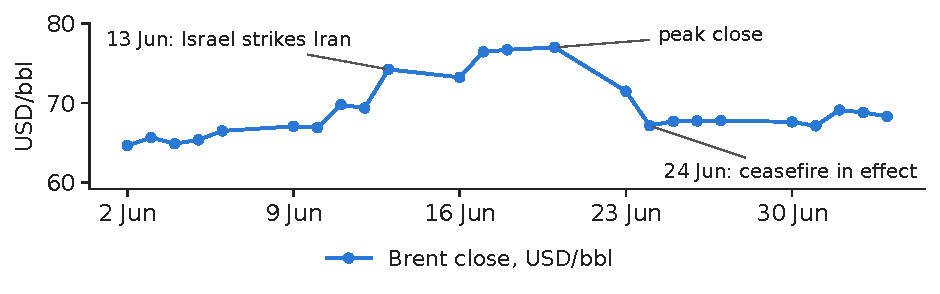
\includegraphics[width=\textwidth,height=0.432\textheight,keepaspectratio]{charts/en/iran_brent.pdf}\end{center}\vspace{-3mm}
\chartsource{Source: Yahoo Finance (BZ=F). Data: 2025-06-02 to 2025-07-04, trading days.}
\vspace{0.5mm}
\begin{itemize}\setlength{\itemsep}{0pt}
  \item Close 12 Jun 2025 69.36 $\to$ 13 Jun (Israel strikes Iran) 74.23: \textbf{\ensuremath{+}7.0\%} (4.3 standard deviations of 2024 daily returns)
    \begin{itemize}\setlength{\itemsep}{0pt}
      \item Peak 77.01 on 20 Jun 2025
      \item 24 Jun (ceasefire in effect) 67.14, i.e.\ \textbf{\ensuremath{-}12.8\%} from the peak and \ensuremath{-}3.2\% vs 12 Jun.
    \end{itemize}
\end{itemize}
\par\vfill\manager{a fuel buyer hedged at the 20 June peak
    \begin{itemize}\setlength{\itemsep}{0pt}
      \item Four days later the market was far below that price.
    \end{itemize}}\par\vspace{0.5mm}
\end{frame}

\subsection{(c) Regional price separation, summer 2024}

\begin{frame}{Case study (c): in July 2024 Romania paid twice the German price}
\framesubtitle{(energy-charts.info; daily and hourly day-ahead prices)\hfill\tryit{notebook \S10c}}
\small
\begin{center}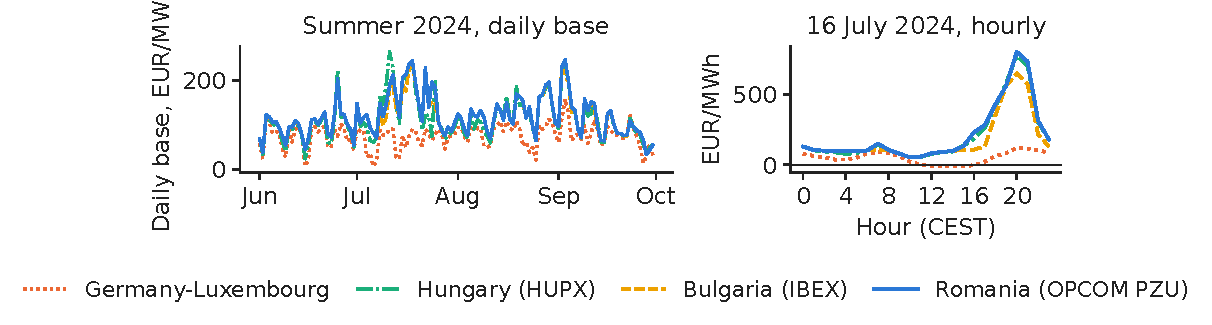
\includegraphics[width=\textwidth,height=0.600\textheight,keepaspectratio]{charts/en/separation_2024.pdf}\end{center}\vspace{-3mm}
\chartsource{Source: energy-charts.info (Fraunhofer ISE); prices from the exchanges OPCOM (RO), IBEX (BG), HUPX (HU), EPEX SPOT (DE-LU), via ENTSO-E. Data: 2024-06-01 to 2024-09-30 daily (left); 2024-07-16 hourly (right).}
\vspace{0.5mm}
\begin{itemize}\setlength{\itemsep}{0pt}
  \item July 2024 averages: RO 145.14, BG 136.47, HU 135.54, DE-LU 67.70 EUR/MWh
    \begin{itemize}\setlength{\itemsep}{0pt}
      \item 16 Jul: RO--DE-LU gap 162.87
      \item RO hourly peak 801.62 at 20:00 while DE-LU was \ensuremath{-}11.48 at 14:00.
    \end{itemize}
\end{itemize}
\par\vfill\manager{for South-East European buyers, the evening hours of hot, dry summers are the main price risk.}\par\vspace{0.5mm}
\end{frame}

\begin{frame}{Case study (c): evening, heat and a congested network}
\framesubtitle{(energy-charts.info; ENTSO-E physical flows)\hfill\tryit{notebook \S10c}}
\small
\begin{columns}[T,onlytextwidth]
\begin{column}{0.60\textwidth}
\begin{itemize}\setlength{\itemsep}{1pt}
  \item Equal prices (within 0.01 EUR/MWh) in July hours: RO--BG 86.8\%, RO--HU 6.3\%, RO--DE-LU 3.1\%
    \begin{itemize}\setlength{\itemsep}{0pt}
      \item The network towards Central Europe was binding
      \item Which element was binding cannot be read from prices alone.
    \end{itemize}
  \item After sunset solar disappears while air conditioning keeps demand high
    \begin{itemize}\setlength{\itemsep}{0pt}
      \item The region must import exactly then.
    \end{itemize}
  \item Romanian hydro in July--August: 1.94 TWh in 2024 vs 2.67 in 2023
    \begin{itemize}\setlength{\itemsep}{0pt}
      \item Net imports averaged 737 MW vs 66 MW.
    \end{itemize}
  \item Summer peak: RO daily 246.89 EUR/MWh on 3 Sep 2024 (DE-LU 158.39)
    \begin{itemize}\setlength{\itemsep}{0pt}
      \item Hourly 1021.61 at 19:00 CEST, the highest Romanian hourly price in our data.
    \end{itemize}
\end{itemize}
\end{column}
\begin{column}{0.37\textwidth}
\begin{block}{Lesson for modelling}
\begin{itemize}\setlength{\itemsep}{1pt}
  \item Coupled prices are equal only while the network is not binding.
  \item Model Romania with regional drivers: hydro, solar, load in South-East Europe.
  \item Treat the spread to Germany as its own, regime-dependent variable.
\end{itemize}
\end{block}
\end{column}
\end{columns}
\end{frame}

\subsection{(d) Negative prices and solar}

\begin{frame}{Case study (d): negative hours cluster in spring, as solar grows year after year}
\framesubtitle{(energy-charts.info; data source: ENTSO-E)\hfill\tryit{notebook \S10d}}
\small
\begin{center}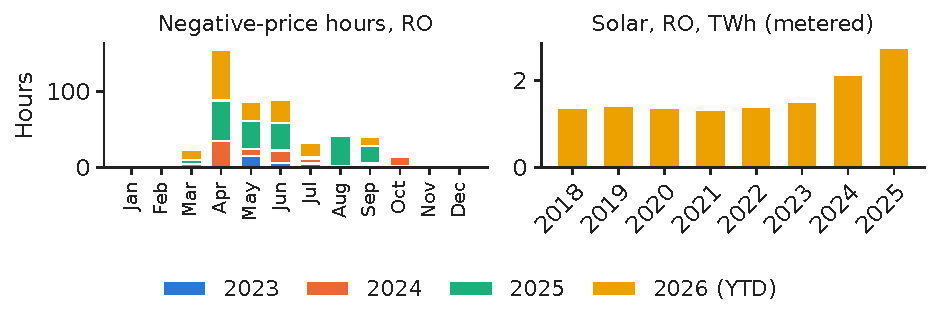
\includegraphics[width=\textwidth,height=0.480\textheight,keepaspectratio]{charts/en/negative_solar.pdf}\end{center}\vspace{-3mm}
\chartsource{Source: energy-charts.info (Fraunhofer ISE); prices from the exchanges OPCOM (RO), IBEX (BG), HUPX (HU), EPEX SPOT (DE-LU), via ENTSO-E. Data: Jan 2023 to 2026-10-31 (left); 2018-2025 (right).}
\vspace{0.5mm}
\begin{itemize}\setlength{\itemsep}{0pt}
  \item April--May hold 49.6\% of Romanian negative hours since 2023 (June--August 34.0\%)
    \begin{itemize}\setlength{\itemsep}{0pt}
      \item Metered solar: 1.46 TWh (2023) $\to$ 2.72 TWh (2025), 4.33 TWh in Jan--Oct 2026.
    \end{itemize}
\end{itemize}
\par\vfill\manager{the cheapest hours are spring weekend middays
    \begin{itemize}\setlength{\itemsep}{0pt}
      \item A battery charges and flexible industry consumes then.
    \end{itemize}}\par\vspace{0.5mm}
\end{frame}

\begin{frame}{Case study (d): what accompanies negative-price days}
\framesubtitle{(own estimation, logit; energy-charts.info)\hfill\tryit{notebook \S10d}}
\footnotesize
\intuition{We describe the realised conditions on days with at least one negative quarter-hour; this describes, it does not forecast for bidding.}
\begin{columns}[T,onlytextwidth]
\begin{column}{0.57\textwidth}
\[ \Pr(\text{negative day})=\Lambda\big(\beta_0+\underbrace{\beta_1R_d}_{\text{residual load}}+\beta_2\mathrm{Hyd}_d+\underbrace{\beta_3\mathrm{Wkd}_d+\gamma_{y}}_{\text{calendar}}\big) \]{\footnotesize\begin{itemize}\setlength{\itemsep}{0pt}
  \item \textbf{\txtwhere}
    \begin{itemize}\setlength{\itemsep}{0pt}
      \item $\Lambda(u)=1/(1+e^{-u})$ (logit)
      \item Residual load $R_d$ = load $-$ solar $-$ wind (daily means, GW), the demand left for other plants
      \item $\gamma_y$ = year effects
      \item Sample 1 Jan 2024 -- 31 Oct 2026, $n=$ 1\,035 days, 108 negative
      \item Full table: Appendix F.
    \end{itemize}
\end{itemize}\par}
\end{column}
\begin{column}{0.40\textwidth}
\begin{itemize}\setlength{\itemsep}{1pt}
  \item \textbf{In plain words}
    \begin{itemize}\setlength{\itemsep}{0pt}
      \item Each extra GW of residual load multiplies the odds of a negative day by 0.24
      \item Each extra GW of hydro multiplies the odds by 4.52
      \item A weekend day multiplies the odds by 16.13
      \item McFadden pseudo-$R^2=$ 0.369
    \end{itemize}
\end{itemize}
\end{column}
\end{columns}
\par\vfill\manager{curtailment of renewables is most likely on spring weekends with full reservoirs.}\par\vspace{0.5mm}
\end{frame}

\subsection{(e) 2026 so far}

\begin{frame}{Case study (e): 2026 prices climbed; oil jumped in March}
\framesubtitle{(energy-charts.info; Yahoo Finance BZ=F; cut-off 31 Oct 2026)\hfill\tryit{notebook \S10e}}
\small
\begin{center}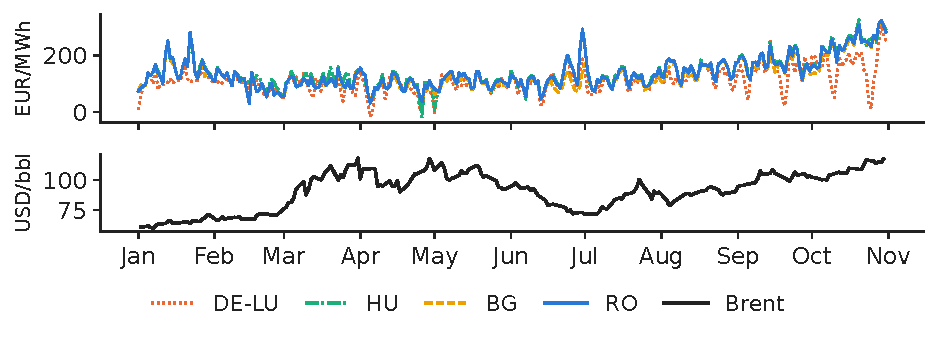
\includegraphics[width=\textwidth,height=0.355\textheight,keepaspectratio]{charts/en/cy_prices.pdf}\end{center}\vspace{-3mm}
\chartsource{Source: energy-charts.info (Fraunhofer ISE); prices from the exchanges OPCOM (RO), IBEX (BG), HUPX (HU), EPEX SPOT (DE-LU), via ENTSO-E. Data: 2026-01-01 to 2026-10-31, daily; Brent: Yahoo Finance (BZ=F).}
\vspace{0.5mm}
\begin{itemize}\setlength{\itemsep}{0pt}
  \item Jan--Oct 2026: Romania 137.45 EUR/MWh (\ensuremath{+}29.8\%)
    \begin{itemize}\setlength{\itemsep}{0pt}
      \item October 239.3 vs 121.9 a year earlier.
    \end{itemize}
  \item Brent monthly average 64.77 $\to$ 108.34 USD/bbl
    \begin{itemize}\setlength{\itemsep}{0pt}
      \item Within March the May contract rose \ensuremath{+}52.2\% (press: conflict involving Iran, Strait of Hormuz)
      \item The \ensuremath{-}14.5\% on 1 April is a contract roll.
    \end{itemize}
\end{itemize}
\par\vfill\manager{budgets set in January were far too low
    \begin{itemize}\setlength{\itemsep}{0pt}
      \item Oil and domestic supply moved the same way.
    \end{itemize}}\par\vspace{0.5mm}
\end{frame}

\begin{frame}{Case study (e): Cernavodă nuclear plant offline twice, hydro below 2025}
\framesubtitle{(Nuclearelectrica, 29 Jul 2026; World Nuclear News, 30 Jul 2026; CNCAN, 9 Sep 2026)\hfill\tryit{notebook \S10e}}
\small
\begin{center}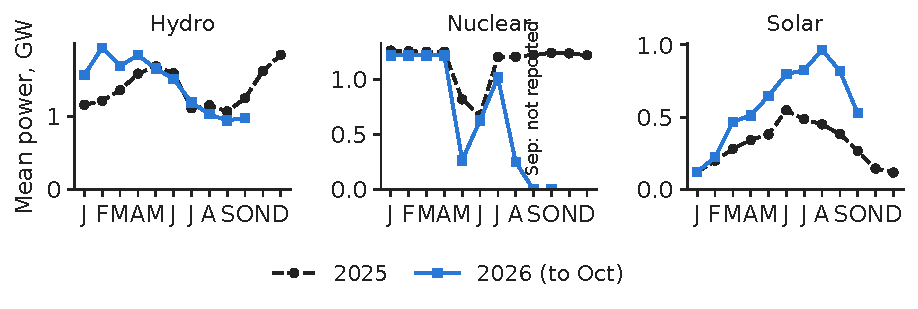
\includegraphics[width=\textwidth,height=0.300\textheight,keepaspectratio]{charts/en/cy_generation.pdf}\end{center}\vspace{-3mm}
\chartsource{Source: energy-charts.info (Fraunhofer ISE); ENTSO-E (Transelectrica data for Romania). Data: monthly means of reported hours, 2025-01 to 2026-10.}
\vspace{0.5mm}
\begin{itemize}\setlength{\itemsep}{0pt}
  \item Nuclear output 0 MW on 19 days in May (data) and from August (Unit 1 shut end-July, Unit 2 on 13 Aug: low Danube)
    \begin{itemize}\setlength{\itemsep}{0pt}
      \item September not reported
      \item Jan--Oct \ensuremath{-}31.3\% on hours reported in both years (lower bound).
    \end{itemize}
  \item Hydro \ensuremath{-}14.7\% in Aug--Oct, solar \ensuremath{+}71.2\% year to date.
\end{itemize}
\par\vfill\manager{one plant can move the national price
    \begin{itemize}\setlength{\itemsep}{0pt}
      \item Read REMIT messages as closely as the weather forecast.
    \end{itemize}}\par\vspace{0.5mm}
\end{frame}

\begin{frame}{Case study (e): 2026 drivers --- price up about 30\%, supply down}
\framesubtitle{(own computation; energy-charts.info)\hfill\tryit{notebook \S10e}}
\small
\begin{center}{\small\renewcommand{\arraystretch}{1.08}\setlength{\tabcolsep}{4pt}
\begin{tabular}{@{}lrrr@{}}\toprule
Jan--Oct & 2025 & 2026 & \% chg \\ \midrule
RO price, EUR/MWh & 105.88 & 137.45 & \cellcolor{Crimson!41}\ensuremath{+}29.8 \\
DE-LU price, EUR/MWh & 87.66 & 114.01 & \cellcolor{Crimson!41}\ensuremath{+}30.1 \\
RO $-$ DE-LU, EUR/MWh & 18.2 & 23.4 &  \\
RO negative hours & 196 & 171.75 &  \\
RO hydro, TWh & 9.61 & 10.44 & \cellcolor{Forest!12}\ensuremath{+}8.6 \\
RO nuclear, TWh$^{*}$ & 7.42 & 5.10 & \cellcolor{Crimson!43}\ensuremath{-}31.3 \\
RO solar, TWh & 2.53 & 4.33 & \cellcolor{Forest!55}\ensuremath{+}71.2 \\
RO net imports, TWh & 3.67 & 2.51 &  \\
\bottomrule\end{tabular}}\end{center}
\vspace{-3mm}
\par\vspace{0.5mm}{\scriptsize \begin{itemize}\setlength{\itemsep}{0pt}
  \item Green = favourable for a consumer, red = unfavourable; cut-off 31 Oct 2026.
  \item $^{*}$Hours reported in both years (lower bound).
\end{itemize}}
\par\vfill\manager{price up by about 30\%, with nuclear, hydro and oil all pointing the same way, and a hedge paid for itself.}\par\vspace{0.5mm}
\end{frame}

\begin{frame}{Case study (e): 2026 extremes in Romania and on Brent}
\framesubtitle{(own computation; energy-charts.info; Yahoo Finance)\hfill\tryit{notebook \S10e}}
\small
\begin{center}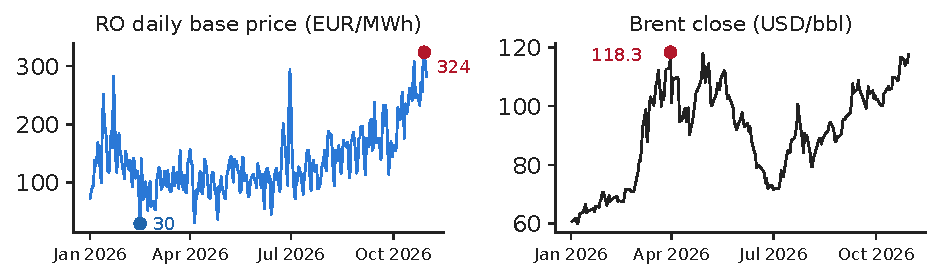
\includegraphics[width=\textwidth,height=0.550\textheight,keepaspectratio]{charts/en/cy_extremes.pdf}\end{center}\vspace{-3mm}
\chartsource{Source: energy-charts.info (OPCOM prices); Yahoo Finance (BZ=F). Data: 2026-01-01 to 2026-10-31, daily.}
\vspace{0.5mm}
\begin{itemize}\setlength{\itemsep}{0pt}
  \item \textbf{Romania}
    \begin{itemize}\setlength{\itemsep}{0pt}
      \item Daily base price: high 323.76 EUR/MWh on 29 Oct 2026, low 29.63 on 15 Feb 2026
      \item Quarter-hour: high 1015.65 on 30 Jun 2026, 18:45, low \ensuremath{-}99.75 on 26 Apr 2026, 13:00 (CET/CEST)
    \end{itemize}
\end{itemize}
\end{frame}

\begin{frame}{Case study (e): 2026 extremes in Germany and on Brent}
\framesubtitle{(own computation; OPCOM SDAC note, 7 May 2026)\hfill\tryit{notebook \S10e}}
\small
\begin{itemize}\setlength{\itemsep}{1pt}
  \item \textbf{Germany}
    \begin{itemize}\setlength{\itemsep}{0pt}
      \item Lowest quarter-hour \ensuremath{-}499.99 on 1 May 2026, 13:15, at the $-500$ floor then in force
      \item After such prices on 26 April and 1 May, the floor became $-600$ for delivery from 29 May 2026
    \end{itemize}
  \item \textbf{Brent}
    \begin{itemize}\setlength{\itemsep}{0pt}
      \item Highest close 118.35 USD/bbl on 31 Mar 2026
      \item Largest daily change excluding contract rolls: \ensuremath{-}13.29\% on 8 Apr 2026
    \end{itemize}
\end{itemize}
\par\vfill\manager{set risk limits on the extremes, not on the averages.}\par\vspace{0.5mm}
\end{frame}

\subsection{(f) Romania, Bulgaria and batteries}

\begin{frame}{Case study (f): since spring 2026, Bulgaria's evenings are cheaper}
\framesubtitle{(energy-charts.info; data source: ENTSO-E; own computation, local time EET)\hfill\tryit{notebook \S10f}}
\small
\begin{center}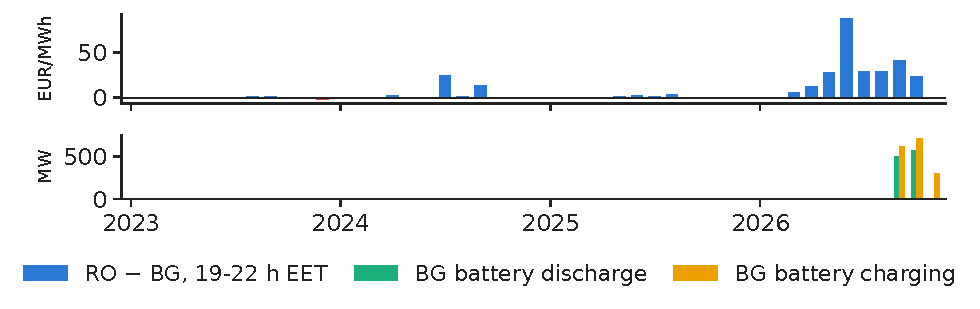
\includegraphics[width=\textwidth,height=0.400\textheight,keepaspectratio]{charts/en/bg_battery.pdf}\end{center}\vspace{-3mm}
\chartsource{Source: energy-charts.info (Fraunhofer ISE); ENTSO-E (Transelectrica data for Romania). Data: 2023-01 to 2026-10, local time; BG battery series reported from 2026-09-10.}
\vspace{0.5mm}
\begin{itemize}\setlength{\itemsep}{0pt}
  \item 19:00--22:00 local time (EET), Apr--Sep, RO vs BG: 171.1 vs 169.7 (2025), 215.5 vs 178.0 EUR/MWh (2026)
    \begin{itemize}\setlength{\itemsep}{0pt}
      \item 2026 middays 11:00--15:00 close (48.1 vs 46.0).
    \end{itemize}
  \item Battery data start only 10 Sep 2026, after the gap opened (May 2026)
    \begin{itemize}\setlength{\itemsep}{0pt}
      \item An association, not proof.
    \end{itemize}
\end{itemize}
\par\vfill\manager{a Romanian battery developer competes for the same regional evening spread (Lecture 6).}\par\vspace{0.5mm}
\end{frame}

\section*{Wrap-up}

\begin{frame}{Quiz 1: counting negative prices}
\small
\begin{itemize}
  \item In a month after 1 October 2025, 48 of Romania's quarter-hour prices were negative
    \begin{itemize}\setlength{\itemsep}{0pt}
      \item A board member asks how many negative hours there were
      \item What do you answer?
    \end{itemize}
\end{itemize}
\vspace{2mm}
\begin{exampleblock}{Answer}
\begin{itemize}
  \item $48\times15/60=12$ hour-equivalents
    \begin{itemize}\setlength{\itemsep}{0pt}
      \item Saying 48 ``hours'' overstates by a factor of 4 against earlier, hourly years
      \item Best answer: ``48 quarter-hours (12 hours)''.
    \end{itemize}
\end{itemize}
\end{exampleblock}
\end{frame}

\begin{frame}{Quiz 2: reading an autocorrelation}
\small
\begin{itemize}
  \item Your analyst says: ``the PZU price autocorrelation is 0.98 at lag 1 and 0.90 at lag 30, so prices are white noise and last month tells us nothing''
    \begin{itemize}\setlength{\itemsep}{0pt}
      \item Is this right?
    \end{itemize}
\end{itemize}
\vspace{2mm}
\begin{exampleblock}{Answer}
\begin{itemize}
  \item No: white noise has autocorrelations near 0
    \begin{itemize}\setlength{\itemsep}{0pt}
      \item Values near 1 mean strong persistence, i.e.\ a unit root or a very slow mean reversion
      \item Run ADF and KPSS and look at the autocorrelation of daily changes.
    \end{itemize}
\end{itemize}
\end{exampleblock}
\end{frame}

\begin{frame}{Wrap-up}
\small
\vspace{-2mm}\begin{multicols}{2}\scriptsize\tableofcontents\end{multicols}
\begin{itemize}\setlength{\itemsep}{1pt}
  \item One auction per day, coupled across Europe, with 96 quarter-hours since Oct 2025
    \begin{itemize}\setlength{\itemsep}{0pt}
      \item Count in hour-equivalents.
    \end{itemize}
  \item Benchmark to beat: the naive forecast (Romania 2025: MAE 22.92 EUR/MWh)
    \begin{itemize}\setlength{\itemsep}{0pt}
      \item Next: forecasting (Lecture 2).
    \end{itemize}
\end{itemize}
\end{frame}

\begin{frame}{Research from our group on the Romanian market}
\framesubtitle{(Bucharest University of Economic Studies; Romanian Academy, Institute for Economic Forecasting)}
\footnotesize
\begin{itemize}\setlength{\itemsep}{1pt}
  \item \textbf{The summer-2024 crisis} (Case c): a counterfactual analysis of Romania's June--July 2024 price crisis on ENTSO-E hourly data
    \begin{itemize}\setlength{\itemsep}{0pt}
      \item A 10\% demand reduction is the robust first-tier intervention, and the peak fell in hours with almost no solar (Andrei, Pele \& Cramer, 2026, PICBE).
    \end{itemize}
  \item \textbf{Explaining price forecasts}: which drivers matter at which horizon (0--6 h up to two weeks) and in which price regime, for Romanian hourly prices 2018--2024 (Andrei, Pele \& Cramer, 2026, PICBE) --- preview of Lecture 7.
  \item \textbf{Forecasting national consumption}: classical seasonal models against neural networks on Romanian load (Proșcanu, Proșcanu, Pele \& Costea, 2025, Romanian J.\ Economic Forecasting) --- preview of Lecture 2.
  \item \textbf{Demand barely reacts to price}: Romanian consumption is price-inelastic
    \begin{itemize}\setlength{\itemsep}{0pt}
      \item Granger causality runs from consumption to price, not back (Proșcanu, Proșcanu \& Pele, 2025, J.\ Social and Economic Statistics) --- why the demand curve is steep.
    \end{itemize}
  \item \textbf{Does liberalisation lower prices?} Causal machine learning on US market liberalisation finds a short-term price decrease of about 7\% (Shahar, Lessmann \& Pele, 2025, arXiv 2507.12331).
\end{itemize}
\par\vspace{0.5mm}{\scriptsize \begin{itemize}\setlength{\itemsep}{0pt}
  \item Findings as stated in the papers' abstracts; numbers on the other slides come from our own data.
\end{itemize}}
\end{frame}

\begin{frame}{Want to learn more?}
\small
\begin{columns}[T,onlytextwidth]
\begin{column}{0.52\textwidth}
\begin{itemize}\setlength{\itemsep}{1pt}
  \item \textbf{R.\ Weron, IIF Distinguished Lectures on electricity price forecasting} (2025): slides \href{https://p.wz.pwr.edu.pl/~weron.rafal/assets/PDF/Weron25_IIF_1.pdf}{part I}, \href{https://p.wz.pwr.edu.pl/~weron.rafal/assets/PDF/Weron25_IIF_2.pdf}{part II}, \href{https://github.com/lipiecki/energy-analytics-2025}{notebooks}, \href{https://www.youtube.com/playlist?list=PLUxduCQo6_X2UTvdP9OE8DwfuBClKFNur}{videos}.
  \item \textbf{epftoolbox}, the open benchmark of Lago et al.\ (2021): \href{https://github.com/jeslago/epftoolbox}{github.com/jeslago/epftoolbox}.
  \item \textbf{Forecasting: Principles and Practice}, 3rd ed.: \href{https://otexts.com/fpp3/}{otexts.com/fpp3}.
\end{itemize}
\end{column}
\begin{column}{0.45\textwidth}
\begin{itemize}\setlength{\itemsep}{1pt}
  \item \textbf{This course}: code, data, notebooks --- \href{https://github.com/danpele/EMQA}{github.com/danpele/EMQA}.
  \item \textbf{Data and rules}: \href{https://www.energy-charts.info}{energy-charts.info}, \href{https://transparency.entsoe.eu}{ENTSO-E Transparency Platform}, \href{https://www.opcom.ro}{opcom.ro}, \href{https://www.transelectrica.ro}{transelectrica.ro}, \href{https://www.jao.eu}{jao.eu}.
  \item \textbf{Experiment yourself}: the notebook reproduces every chart and number of this lecture --- \href{\emqarepo/\emqanb}{notebooks/}.
\end{itemize}
\end{column}
\end{columns}
\end{frame}

\begin{frame}{References (1/2)}
\scriptsize
\begin{itemize}\setlength{\itemsep}{0pt}\scriptsize
\item Andrei, A.-V., Pele, D.-T.\ \& Cramer, A.-A.\ (2026). Evaluating intervention effectiveness during extreme price events: A counterfactual analysis of Romania's 2024 energy crisis. \textit{Proceedings of the International Conference on Business Excellence}, 20(1), 84--103. \href{https://doi.org/10.2478/picbe-2026-0013}{doi:10.2478/picbe-2026-0013}
\item Andrei, A.-V., Pele, D.-T.\ \& Cramer, A.-A.\ (2026). Multi-horizon explainability in energy price forecasting: Disentangling market dynamics and renewable intermittency in Romania's liberalized electricity market. \textit{Proceedings of the International Conference on Business Excellence}, 20(1), 104--117. \href{https://doi.org/10.2478/picbe-2026-0014}{doi:10.2478/picbe-2026-0014}
\item Cleveland, R.\,B., Cleveland, W.\,S., McRae, J.\,E.\ \& Terpenning, I.\ (1990). STL: A seasonal-trend decomposition procedure based on loess. \textit{Journal of Official Statistics}, 6(1), 3--73.
\item Dickey, D.\,A.\ \& Fuller, W.\,A.\ (1979). Distribution of the estimators for autoregressive time series with a unit root. \textit{Journal of the American Statistical Association}, 74(366), 427--431. \href{https://doi.org/10.1080/01621459.1979.10482531}{doi:10.1080/01621459.1979.10482531}
\item Hyndman, R.\,J.\ \& Athanasopoulos, G.\ (2021). \textit{Forecasting: Principles and Practice}, 3rd ed. OTexts.
\item Janczura, J., Trück, S., Weron, R.\ \& Wolff, R.\,C.\ (2013). Identifying spikes and seasonal components in electricity spot price data: A guide to robust modeling. \textit{Energy Economics}, 38, 96--110. \href{https://doi.org/10.1016/j.eneco.2013.03.013}{doi:10.1016/j.eneco.2013.03.013}
\item Jarque, C.\,M.\ \& Bera, A.\,K.\ (1980). Efficient tests for normality, homoscedasticity and serial independence of regression residuals. \textit{Economics Letters}, 6(3), 255--259. \href{https://doi.org/10.1016/0165-1765(80)90024-5}{doi:10.1016/0165-1765(80)90024-5}
\item Kwiatkowski, D., Phillips, P.\,C.\,B., Schmidt, P.\ \& Shin, Y.\ (1992). Testing the null hypothesis of stationarity against the alternative of a unit root. \textit{Journal of Econometrics}, 54(1--3), 159--178. \href{https://doi.org/10.1016/0304-4076(92)90104-Y}{doi:10.1016/0304-4076(92)90104-Y}
\item Lago, J., Marcjasz, G., De Schutter, B.\ \& Weron, R.\ (2021). Forecasting day-ahead electricity prices: A review of state-of-the-art algorithms, best practices and an open-access benchmark. \textit{Applied Energy}, 293, 116983. \href{https://doi.org/10.1016/j.apenergy.2021.116983}{doi:10.1016/j.apenergy.2021.116983}
\item Ljung, G.\,M.\ \& Box, G.\,E.\,P.\ (1978). On a measure of lack of fit in time series models. \textit{Biometrika}, 65(2), 297--303. \href{https://doi.org/10.1093/biomet/65.2.297}{doi:10.1093/biomet/65.2.297}
\item Maciejowska, K., Uniejewski, B.\ \& Weron, R.\ (2023). Forecasting electricity prices. \textit{Oxford Research Encyclopedia of Economics and Finance}. \href{https://doi.org/10.1093/acrefore/9780190625979.013.667}{doi:10.1093/acrefore/9780190625979.013.667}
\end{itemize}
\end{frame}

\begin{frame}{References (2/2)}
\scriptsize
\begin{itemize}\setlength{\itemsep}{0pt}\scriptsize
\item MacKinnon, J.\,G.\ (1996). Numerical distribution functions for unit root and cointegration tests. \textit{Journal of Applied Econometrics}, 11(6), 601--618.
\item Nogales, F.\,J., Contreras, J., Conejo, A.\,J.\ \& Espínola, R.\ (2002). Forecasting next-day electricity prices by time series models. \textit{IEEE Transactions on Power Systems}, 17(2), 342--348. \href{https://doi.org/10.1109/TPWRS.2002.1007902}{doi:10.1109/TPWRS.2002.1007902}
\item Proșcanu, C.\,A., Proșcanu, M.\,E., Pele, D.\,T.\ \& Costea, A.\ (2025). Watt's next? Benchmarking time series models on Romania's national electricity consumption. \textit{Romanian Journal of Economic Forecasting}, issue 3, 146--163.
\item Proșcanu, C., Proșcanu, M.\ \& Pele, D.\,T.\ (2025). The price elasticity of electricity demand in Romania. \textit{Journal of Social and Economic Statistics}, 14(2), 131--141. \href{https://doi.org/10.2478/jses-2025-0009}{doi:10.2478/jses-2025-0009}
\item Said, S.\,E.\ \& Dickey, D.\,A.\ (1984). Testing for unit roots in autoregressive-moving average models of unknown order. \textit{Biometrika}, 71(3), 599--607. \href{https://doi.org/10.1093/biomet/71.3.599}{doi:10.1093/biomet/71.3.599}
\item Shahar, O., Lessmann, S.\ \& Pele, D.\,T.\ (2025). Causality analysis of electricity market liberalization on electricity price using novel machine learning methods. arXiv:2507.12331.
\item Uniejewski, B., Weron, R.\ \& Ziel, F.\ (2018). Variance stabilizing transformations for electricity spot price forecasting. \textit{IEEE Transactions on Power Systems}, 33(2), 2219--2229. \href{https://doi.org/10.1109/TPWRS.2017.2734563}{doi:10.1109/TPWRS.2017.2734563}
\item Weron, R.\ (2014). Electricity price forecasting: A review of the state-of-the-art with a look into the future. \textit{International Journal of Forecasting}, 30(4), 1030--1081. \href{https://doi.org/10.1016/j.ijforecast.2014.08.008}{doi:10.1016/j.ijforecast.2014.08.008}
\item Ziel, F.\ \& Weron, R.\ (2018). Day-ahead electricity price forecasting with high-dimensional structures: Univariate vs.\ multivariate modeling frameworks. \textit{Energy Economics}, 70, 396--420. \href{https://doi.org/10.1016/j.eneco.2017.12.016}{doi:10.1016/j.eneco.2017.12.016}
\item Market and event sources: OPCOM press releases (19 Nov 2019; 27 Oct 2021; 19 Mar 2025; 1 Oct 2025) and SDAC note (7 May 2026, minimum price $-600$ from delivery 29 May 2026); Nuclearelectrica current report (29 Jul 2026); World Nuclear News (30 Jul 2026); statement of the National Commission for Nuclear Activities Control (CNCAN) on Cernavodă (9 Sep 2026); press reports (Mar 2026) on the Strait of Hormuz.
\end{itemize}
\end{frame}

\appendix

\section*{Appendix}

\begin{frame}{Appendix A: ADF and KPSS in full}
\small
\begin{columns}[T,onlytextwidth]
\begin{column}{0.49\textwidth}
\begin{block}{ADF (Said \& Dickey, 1984)}
\[ \Delta x_t=\alpha+\beta t+\gamma x_{t-1}+\sum_{j=1}^{p}\delta_j\Delta x_{t-j}+u_t \]\begin{itemize}\setlength{\itemsep}{1pt}
  \item $H_0:\gamma=0$ vs $H_1:\gamma<0$
    \begin{itemize}\setlength{\itemsep}{0pt}
      \item $\tau=\hat\gamma/\mathrm{se}(\hat\gamma)$ follows the Dickey--Fuller distribution
      \item $p$-values from MacKinnon (1996).
    \end{itemize}
  \item Lag order: minimise AIC starting from $p_{\max}=12(T/100)^{1/4}$.
  \item Deterministic terms must match the alternative
    \begin{itemize}\setlength{\itemsep}{0pt}
      \item Constant: level-stationary
      \item Trend: trend-stationary.
    \end{itemize}
\end{itemize}
\end{block}
\end{column}
\begin{column}{0.49\textwidth}
\begin{block}{KPSS (Kwiatkowski et al., 1992)}
\[ \mathrm{KPSS}=\frac{1}{T^2\hat\sigma^2_{\mathrm{LR}}}\sum_{t=1}^T S_t^2,\quad S_t=\sum_{s\le t}e_s \]\[ \hat\sigma^2_{\mathrm{LR}}=\hat\gamma_0+2\sum_{k=1}^{\ell}\Big(1-\frac{k}{\ell+1}\Big)\hat\gamma_k \]\begin{itemize}\setlength{\itemsep}{1pt}
  \item $e_s$ = residuals from a regression on a constant (and trend).
  \item Bartlett kernel with bandwidth $\ell$ (Hobijn et al.\ rule in statsmodels)
    \begin{itemize}\setlength{\itemsep}{0pt}
      \item Critical value 0.463 (5\%, level).
    \end{itemize}
\end{itemize}
\end{block}
\end{column}
\end{columns}
\end{frame}

\begin{frame}{Appendix B: classical decomposition, worked example}
\small
\begin{columns}[T,onlytextwidth]
\begin{column}{0.56\textwidth}
\[ \hat T_t=\tfrac{1}{24}x_{t-6}+\tfrac{1}{12}\textstyle\sum_{j=-5}^{5}x_{t+j}+\tfrac{1}{24}x_{t+6} \]\begin{itemize}\setlength{\itemsep}{1pt}
  \item First trend value, Jul 2016: $\hat T=\frac{1}{24}(7.424+7.870)+\frac{1}{12}\cdot 72.503=$ 6.679 GW (Jan 2016 and Jan 2017 at half weight; Feb--Dec 2016 summed).
  \item Observed 6.389 GW $\Rightarrow$ deviation \ensuremath{-}0.290.
  \item Seasonal index: $\hat S_j=\bar d_j-\frac1{12}\sum_i\bar d_i$ (raw means summed to 0.0005).
\end{itemize}
\end{column}
\begin{column}{0.40\textwidth}
{\footnotesize\renewcommand{\arraystretch}{1.2}\setlength{\tabcolsep}{4pt}
\begin{tabular}{@{}lr@{\hspace{6mm}}lr@{}}\toprule
Month & $\hat S_j$ & Month & $\hat S_j$ \\ \midrule
Jan & 0.686 & Jul & \ensuremath{-}0.143 \\
Feb & 0.694 & Aug & \ensuremath{-}0.302 \\
Mar & 0.237 & Sep & \ensuremath{-}0.444 \\
Apr & \ensuremath{-}0.381 & Oct & \ensuremath{-}0.194 \\
May & \ensuremath{-}0.650 & Nov & 0.374 \\
Jun & \ensuremath{-}0.442 & Dec & 0.565 \\
\bottomrule\end{tabular}}
\par\vspace{0.5mm}{\scriptsize \begin{itemize}\setlength{\itemsep}{0pt}
  \item Romanian load (GW), Jan 2016 -- Dec 2025; checked against statsmodels.
\end{itemize}}
\end{column}
\end{columns}
\end{frame}

\begin{frame}{Appendix C: the STL algorithm}
\framesubtitle{(Cleveland, Cleveland, McRae \& Terpenning, 1990, JOS)}
\small
\begin{itemize}\setlength{\itemsep}{1pt}
  \item \textbf{Inner loop} (repeated): (1) detrend, $x_t-\hat T_t$
    \begin{itemize}\setlength{\itemsep}{0pt}
      \item (2) smooth each month's sub-series (all Januaries, all Februaries, \dots) by loess with span $n_s$
      \item (3) remove its low-frequency part $\Rightarrow\hat S_t$
      \item (4) smooth $x_t-\hat S_t$ by loess with span $n_t$ $\Rightarrow\hat T_t$.
    \end{itemize}
  \item \textbf{Outer loop}: robustness weights $\rho_t=B\big(|\hat R_t|/(6\,\mathrm{median}|\hat R|)\big)$, $B(u)=(1-u^2)^2$ for $|u|<1$, else 0, so outliers count less in the next inner loop.
  \item Here: period 12, $n_s=13$, robust
    \begin{itemize}\setlength{\itemsep}{0pt}
      \item Strength of seasonality $1-\Var(R)/\Var(S+R)=$ 0.848.
    \end{itemize}
  \item Additive only: for multiplicative seasonality apply STL to $\ln x_t$ (or asinh for prices).
\end{itemize}
\end{frame}

\begin{frame}{Appendix D: generation mix in numbers}
\framesubtitle{(energy-charts.info; data source: ENTSO-E)}
\small
\begin{center}{\footnotesize\renewcommand{\arraystretch}{1.1}\setlength{\tabcolsep}{4pt}
\begin{tabular}{@{}lrrrrrrr@{}}\toprule
Share, \% & 2015 & 2020 & 2023 & 2024 & 2025 & Jan--Oct 2025 & Jan--Oct 2026 \\ \midrule
Hydro & \cellcolor{MainBlue!36}26.2 & \cellcolor{MainBlue!39}27.8 & \cellcolor{MainBlue!45}\textcolor{white}{32.4} & \cellcolor{MainBlue!39}27.9 & \cellcolor{MainBlue!36}25.6 & \cellcolor{MainBlue!36}25.7 & \cellcolor{MainBlue!38}27.6 \\
Nuclear & \cellcolor{MainBlue!38}17.9 & \cellcolor{MainBlue!44}\textcolor{white}{20.7} & \cellcolor{MainBlue!42}\textcolor{white}{19.8} & \cellcolor{MainBlue!45}\textcolor{white}{21.1} & \cellcolor{MainBlue!45}\textcolor{white}{21.3} & \cellcolor{MainBlue!42}\textcolor{white}{19.8} & \cellcolor{MainBlue!29}13.5 \\
Coal & \cellcolor{MainBlue!45}\textcolor{white}{28.3} & \cellcolor{MainBlue!28}17.4 & \cellcolor{MainBlue!23}14.4 & \cellcolor{MainBlue!22}13.6 & \cellcolor{MainBlue!22}13.8 & \cellcolor{MainBlue!23}14.4 & \cellcolor{MainBlue!19}12.1 \\
Gas & \cellcolor{MainBlue!32}14.6 & \cellcolor{MainBlue!40}18.4 & \cellcolor{MainBlue!37}16.9 & \cellcolor{MainBlue!44}\textcolor{white}{20.1} & \cellcolor{MainBlue!44}\textcolor{white}{20.2} & \cellcolor{MainBlue!43}\textcolor{white}{19.8} & \cellcolor{MainBlue!45}\textcolor{white}{20.5} \\
Wind & \cellcolor{MainBlue!33}10.3 & \cellcolor{MainBlue!40}12.4 & \cellcolor{MainBlue!43}\textcolor{white}{13.2} & \cellcolor{MainBlue!40}12.4 & \cellcolor{MainBlue!40}12.4 & \cellcolor{MainBlue!41}\textcolor{white}{12.6} & \cellcolor{MainBlue!45}\textcolor{white}{13.9} \\
Solar & \cellcolor{MainBlue!8}1.9 & \cellcolor{MainBlue!9}2.4 & \cellcolor{MainBlue!10}2.6 & \cellcolor{MainBlue!16}4.1 & \cellcolor{MainBlue!22}5.7 & \cellcolor{MainBlue!27}6.8 & \cellcolor{MainBlue!45}\textcolor{white}{11.4} \\
Biomass & \cellcolor{MainBlue!36}0.8 & \cellcolor{MainBlue!40}0.9 & \cellcolor{MainBlue!31}0.7 & \cellcolor{MainBlue!40}0.9 & \cellcolor{MainBlue!40}0.9 & \cellcolor{MainBlue!40}0.9 & \cellcolor{MainBlue!45}\textcolor{white}{1.0} \\
\textbf{Total TWh} & 64.2 & 55.4 & 56.6 & 51.2 & 47.4 & 37.4 & 37.9 \\
Load TWh & 57.0 & 58.1 & 53.4 & 54.3 & 53.6 & 43.9 & 42.3 \\
Net imp. TWh & \ensuremath{-}6.9 & 1.9 & \ensuremath{-}3.1 & 3.0 & 3.8 & 3.7 & 2.5 \\
\bottomrule\end{tabular}}
\par\vspace{0.5mm}{\scriptsize \begin{itemize}\setlength{\itemsep}{0pt}
  \item Last two columns: hours reported in both years.
  \item Net imports $>0$: into Romania.
\end{itemize}}\end{center}
\end{frame}

\begin{frame}{Appendix E: naive benchmark, all years}
\framesubtitle{(Nogales et al., 2002, IEEE TPWRS; Weron, 2014, IJF)}
\small
\begin{center}{\footnotesize\renewcommand{\arraystretch}{1.1}\setlength{\tabcolsep}{4pt}
\begin{tabular}{@{}lrrrrrrrr@{}}\toprule
MAE & 2019 & 2020 & 2021 & 2022 & 2023 & 2024 & 2025 & 2026 \\ \midrule
RO naive & \cellcolor{Forest!55}9.7 & \cellcolor{Forest!55}7.4 & \cellcolor{Forest!55}19.9 & \cellcolor{Forest!47}59.7 & \cellcolor{Forest!55}26.0 & \cellcolor{Forest!55}27.7 & \cellcolor{Forest!55}22.9 & \cellcolor{Forest!55}29.4 \\
RO $d-1$ & \cellcolor{Crimson!19}10.7 & \cellcolor{Crimson!14}8.1 & \cellcolor{Forest!5}22.2 & \cellcolor{Forest!55}58.5 & \cellcolor{Forest!27}27.3 & \cellcolor{Forest!20}29.7 & \cellcolor{Forest!14}24.9 & \cellcolor{Forest!29}31.1 \\
RO $d-7$ & \cellcolor{Crimson!55}11.2 & \cellcolor{Crimson!55}8.6 & \cellcolor{Crimson!55}25.1 & \cellcolor{Crimson!55}75.4 & \cellcolor{Crimson!55}31.0 & \cellcolor{Crimson!55}33.9 & \cellcolor{Crimson!55}28.2 & \cellcolor{Crimson!55}36.6 \\
DE-LU naive & \cellcolor{Forest!15}9.8 & \cellcolor{Forest!55}9.3 & \cellcolor{Forest!55}24.3 & \cellcolor{Forest!25}66.2 & \cellcolor{Forest!31}28.6 & \cellcolor{Forest!55}27.3 & \cellcolor{Forest!31}27.5 & \cellcolor{Forest!16}36.1 \\
DE-LU $d-1$ & \cellcolor{Forest!55}9.5 & \cellcolor{Crimson!20}10.0 & \cellcolor{Forest!40}25.3 & \cellcolor{Forest!55}58.2 & \cellcolor{Forest!55}27.2 & \cellcolor{Forest!44}27.8 & \cellcolor{Forest!55}26.0 & \cellcolor{Forest!55}32.8 \\
DE-LU $d-7$ & \cellcolor{Crimson!55}10.3 & \cellcolor{Crimson!55}10.3 & \cellcolor{Crimson!55}31.5 & \cellcolor{Crimson!55}87.1 & \cellcolor{Crimson!55}33.6 & \cellcolor{Crimson!55}32.8 & \cellcolor{Crimson!55}32.8 & \cellcolor{Crimson!55}42.2 \\
\bottomrule\end{tabular}}\end{center}
\par\vspace{0.5mm}{\scriptsize \begin{itemize}\setlength{\itemsep}{0pt}
  \item MAE in EUR/MWh on hourly prices (from Oct 2025: hourly mean of the 15-min prices).
  \item Green = best of the three in that year and zone.
\end{itemize}}
\end{frame}

\begin{frame}{Appendix F: fat tails and the negative-day logit in full}
\framesubtitle{(Jarque \& Bera, 1980; own estimation)}
\small
\begin{columns}[T,onlytextwidth]
\begin{column}{0.43\textwidth}
\[ \hat S=\frac{\frac1T\sum_t(r_t-\bar r)^3}{\hat\sigma^3},\quad \hat K=\frac{\frac1T\sum_t(r_t-\bar r)^4}{\hat\sigma^4} \]\[ \mathrm{JB}=\frac T6\Big(\hat S^2+\frac{(\hat K-3)^2}{4}\Big)\sim\chi^2_2 \]\begin{itemize}\setlength{\itemsep}{1pt}
  \item Brent daily log returns (roll days removed): skewness \ensuremath{-}0.94, excess kurtosis 13.98, JB 23\,500 (5\% critical value 5.99)
    \begin{itemize}\setlength{\itemsep}{0pt}
      \item Student-$t$ fit: 3.21 degrees of freedom.
    \end{itemize}
\end{itemize}
\end{column}
\begin{column}{0.54\textwidth}
{\footnotesize\renewcommand{\arraystretch}{1.1}\setlength{\tabcolsep}{4pt}
\begin{tabular}{@{}lrrr@{}}\toprule
 & $\hat\beta$ & odds ratio & $z$ \\ \midrule
Constant & \ensuremath{-}0.023 & 0.98 & \ensuremath{-}0.02 \\
Residual load, GW & \ensuremath{-}1.445 & 0.24 & \ensuremath{-}7.67 \\
Hydro, GW & 1.508 & 4.52 & 4.37 \\
Weekend & 2.780 & 16.13 & 9.24 \\
Year 2025 & 1.337 & 3.81 & 3.98 \\
Year 2026 & 0.534 & 1.71 & 1.54 \\
\bottomrule\end{tabular}}
\par\vspace{0.5mm}{\scriptsize \begin{itemize}\setlength{\itemsep}{0pt}
  \item Logit for a day with at least one negative RO quarter-hour; base year 2024.
\end{itemize}}
\end{column}
\end{columns}
\end{frame}

\begin{frame}{Appendix G: converting gas and oil prices to EUR/MWh}
\framesubtitle{(World Bank Commodity Price Data; ECB reference rates)}
\small
\begin{columns}[T,onlytextwidth]
\begin{column}{0.50\textwidth}
\[ P^{\text{EUR/MWh}}=P^{\text{USD/MMBtu}}\times 3.412142\,/\,e_m \]{\footnotesize\begin{itemize}\setlength{\itemsep}{0pt}
  \item \textbf{\txtwhere}
    \begin{itemize}\setlength{\itemsep}{0pt}
      \item $1\ \text{MMBtu}=0.293071$ MWh, so $1/0.293071=3.412142$ MMBtu per MWh
      \item $e_m$ = monthly USD per EUR rate of the ECB
      \item Brent: 1 bbl = 159 litres, quoted in USD/bbl
    \end{itemize}
\end{itemize}\par}
\end{column}
\begin{column}{0.47\textwidth}
\begin{itemize}\setlength{\itemsep}{1pt}
  \item World Bank TTF is a monthly average in USD/MMBtu converted with the ECB rate
    \begin{itemize}\setlength{\itemsep}{0pt}
      \item It is not a traded EUR quote.
    \end{itemize}
  \item Compare fuels and power only in the same unit and currency
    \begin{itemize}\setlength{\itemsep}{0pt}
      \item A gas price in USD/MMBtu and a power price in EUR/MWh differ by a factor of about 3.4 before any exchange rate.
    \end{itemize}
\end{itemize}
\end{column}
\end{columns}
\end{frame}

\end{document}
